\cotefile{97}
\scanpage{19}\mspage{- IV- \handwritten{1102} -}
(21.6.5) Considérons donc un diviseur \uline{positif} $\unsure{D'|D}$ sur $X$\inserted{ ($X$ é\deleted{\unsure{n}}tant supposé \uline{noethérien})}, de sorte que l'Idéal \inserted{fractionnaire} $\underline I_{X}(D)$ est un \uline{Idéal de} $\underline O_{X}$, qui est un $\underline O_{X}$-Module \uline{inversible}; soit $Y(D)$ le sous-préschéma fermé de $X$ qu'il définit. \deleted{\unsure{Cela signifie}}\inserted{Pour} \deleted{\unsure{en|qu}} tout $x\handwritten{\in}Y(D)$, \deleted{\unsure{que,}} il y a par hypothèse un voisinage \inserted{\handwritten{ouvert}} $U$ de $x$ dans $X$ et une section \uline{régulière} $t\handwritten{\in\Gamma}(U,\underline O_{X})$ telle que $\underline I_{X}(D)\handwritten{\mid}U=\underline O_{U}\mathbin{.}t$ (21.2.7) ; en d'autres termes, l'immersion canonique $Y(D)\handwritten{\to}X$ est \uline{régulière et de codimension 1} \inserted{(19.1.4) en tout point de $Y( D)$}. On notera d'ailleurs qu'inversement, si $Y$ \reversemarginpar
% slanted
\margin{\figure{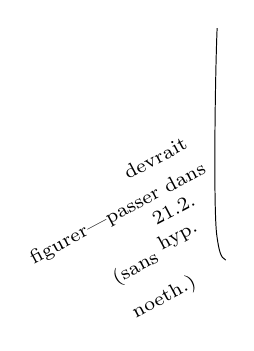
\begin{tikzpicture}[x=1em,y=1em,baseline=0pt]
  \node[anchor=east,rotate=28,inner sep=0pt,font=\scriptsize] at (-.7,1.2)
    {\handwritten{\unsure{devrait}}};
  \node[anchor=east,rotate=28,inner sep=0pt,font=\scriptsize] at (0,.25)
    {\handwritten{\unsure{figurer|passer} dans}};
  \node[anchor=east,rotate=28,inner sep=0pt,font=\scriptsize] at (-.4,-.85)
    {\handwritten{21.2.}};
  \node[anchor=east,rotate=28,inner sep=0pt,font=\scriptsize] at (-.3,-1.85)
    {\handwritten{hyp.}};
  \node[anchor=east,rotate=28,inner sep=0pt,font=\scriptsize] at (-1.7,-2.95)
    {\handwritten{(sans}};
  \node[anchor=east,rotate=28,inner sep=0pt,font=\scriptsize] at (-.35,-3.85)
    {\handwritten{noeth.)}};
  \draw[line width=.35pt] (.43,5.3) .. controls (.36,3.7) and (.29,-1.3) .. (.42,-2.2)
     .. controls (.49,-2.7) and (.55,-3) .. (.74,-3.08);
\end{tikzpicture}}}
est un sous-préschéma fermé de $X$, régulièrement immergé dans $X$ et \deleted{\unsure{est}} de codimension $1$ en tout point de $Y$, il existe un diviseur positif et un seul \deleted{\unsure{positif|préschéma}} $D$ sur $X$ tel que $Y(D)=Y$, car\deleted{\unsure{ cela signifie}}\inserted{ pour} \deleted{\unsure{en|qu}} tout $x\handwritten{\in}Y$, il y a un voisinage $U$ de $x$ dans $X$ tel que $Y\handwritten{\cap}U$ soit défini par un Idéal de $\underline{\mathbb O}_{U}$ de la forme $\underline O_{U}\mathbin{.}t$, où $t$ est \uline{réguli\deleted{\unsure{re}}\handwritten{\unsure{er}}} dans $\handwritten{\Gamma}(U,\underline O_{X})$.


Puisque $X$ est supposé noethérien, $Y(D)$ n'a qu'un nombre fini de points maximaux, et en chacun de ces points $x$, on a $\operatorname{codim}(\handwritten{\{}x\handwritten{\}},X)={}\allowbreak{}=\operatorname{dim}(\underline O_{X,x})=1$, autrement dit $x\handwritten{\in}X^{(1)}$ ;
% slanted
\margin{\handwritten{\uline{réf} !}}\normalmarginpar
\deleted{\illegible{2} \unsure{partie} \illegible{1}} en outre, $\underline O_{Y(D),x}$ est un anneau \uline{artinien} en chacun de ces poi\deleted{g}nts. En tout point $x\handwritten{\in}X^{(1)}$ qui n'est pas point maximal de $Y(D)$, on a nécessairement $x\handwritten{\notin}Y(D)$, donc $\underline O_{Y(D),x}=0$. Posons
\[
  \operatorname{cyc}(D)=\handwritten{\sum}^{\handwritten{\unsure{\prime}}}_{x\handwritten{\in}X^{(1)}}
  \operatorname{long}(\underline O_{Y(D),x})\mathbin{.}\handwritten{\overline}{\handwritten{\{}x\handwritten{\}}}
  \tag*{(21.6.5.1)}
\]
qui est donc un élément de $Z^{1}\llap{\raisebox{-.12ex}[0pt][0pt]{\tiny\unsure{.}}}(X)$.

\uline{Proposition} (21.6.6) .- \deleted{\uline{Si} $X$ \uline{est noethérien}}, \uline{\deleted{l}\handwritten{L}'application} $D\handwritten{\leadsto}\operatorname{cyc}(D)$\deleted{\unsure{;}} \uline{est un homomorphisme du monoïde} $\operatorname{Div}^{+}(X)$ \uline{dans} $Z^{1}(X)$ .

Tout revient à voir que pour deux diviseurs \uline{positifs} $D,D'$, on a $\operatorname{cyc}(D+D')=\operatorname{cyc}(D)+\operatorname{cyc}(D')$. Or, on a (21.2.5) $\underline I_{X}(D+D')=\underline I_{X}(D)\underline I_{X}(D')$; tout revient à voir que si $x\handwritten{\in}X^{(1)}$, \inserted{\handwritten{si l'on pose}} $A=\underline O_{X,x}$, et si $t$ et $t'$ sont deux éléments réguliers de $A$, on a $\operatorname{long}(A/tt'A)=\operatorname{long}(A/tA)+{}\allowbreak{}+\operatorname{long}(A/t'A)$ ; mais puisque \deleted{\unsure{$x$}} $t$ est régulier, $tA/tt'A$ est isomorphe à $A/t'A$, d'où \deleted{\unsure{résulte}} aussitôt la proposition.

Il résulte aussitôt des définitions que pour tout ouvert $U\handwritten{\subset}X$, on
% archive sheet number: 18

\cotefile{123}
\scanpage{2}
Compléments sur transformation de Coxeter d'un système de racines\inserted{\handwritten{
\begin{tikzpicture}[baseline=(word.base)]
  \node[inner sep=1pt] (word) {\unsure{irréductible|irreductible}};
  \draw (word.center) ellipse (1.05cm and 0.24cm);
  \draw ([xshift=-0.55cm]word.south) .. controls +(-0.10,-0.18) and +(-0.04,0.16) .. ++(-0.12,-0.38);
\end{tikzpicture}}} (Kostant).
% The circled insertion is above the end of the title; its leader ends before (Kostant).
\par\noindent\hspace*{1.5cm}\handwritten{The principal 3-dimensional subgroup \unsure{....|...}\quad th. 9.2.}
% The English reference is written immediately below the title, not in a side margin.

a) Soit $w\handwritten{\in}W$. Alors toute valeur propre de $w$ \unsure{est} une racine de $1$ d'ordre divisant un des entiers $m_i+1$ (où les $m_i$ sont les exposants caractéristiques), donc d'ordre $\handwritten{\leq}h$. Pour qu'il y en ait une qui soit d'ordre $h$, il faut et suffit que $w$ soit une transformation de Coxeter, et\inserted{alors} les éléments non nuls du sous-espace propre correspondant\handwritten{$_\circ$}\reversemarginpar
\margin{\inserted{\handwritten{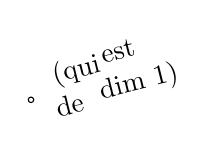
\begin{tikzpicture}[x=1cm,y=1cm]
  \draw (-0.18,-0.12) circle (0.035);
  \node[anchor=base west,rotate=14] at (0,0.06) {(qui};
  \node[anchor=base west,rotate=14] at (0.62,0.31) {est};
  \node[anchor=base west,rotate=14] at (0.05,-0.37) {de};
  \node[anchor=base west,rotate=14] at (0.60,-0.14) {dim $1$)};
\end{tikzpicture}}}}\normalmarginpar
% Left marginal insertion: est stands above/right of (qui; de stands lower/left of dim 1).
sont des éléments réguliers.
\margin{\handwritten{\figure{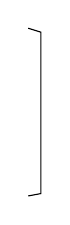
\begin{tikzpicture}[x=1cm,y=1cm]\draw (-0.16,0.05)--(0,0)--(0,-2.05)--(-0.16,-2.08);\end{tikzpicture}}}}

\uline{Corollaire}\handwritten{1}: Soit $\handwritten{\mu}$ le sous-groupe de $W$ engendré par un élément de Coxeter $c$, donc $\handwritten{\mu\simeq}\underline{Z}\handwritten{/}h\underline{Z}$. Alors $\handwritten{\mu}$ est égal au centralisateur de $c$, donc de $\handwritten{\mu}$, et si $\handwritten{\nu}$ est le normalisateur de $\handwritten{\mu}$, l'homomorphisme
\reversemarginpar\margin{\handwritten{\figure{\begin{tikzpicture}[x=1cm,y=1cm]\draw (0,0)--(0,-2.4);\end{tikzpicture}}}}\normalmarginpar
\[
\handwritten{\unsure{\psi|\nu}/\mu\longrightarrow}\operatorname{Aut}(\handwritten{\mu})\handwritten{\simeq}(\underline{Z}/h\underline{Z})^{\handwritten{*}}
\]
\margin{\handwritten{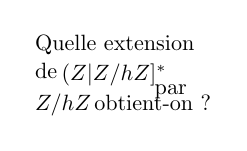
\begin{tikzpicture}[x=1cm,y=1cm,scale=0.80,transform shape]
  \node[anchor=base west] at (0,0.95) {Quelle extension};
  \node[anchor=base west] at (0,0.50) {de};
  \node[anchor=base west] at (0.42,0.48) {$(\unsure{Z|\mathbb{Z}}/hZ]^*$};
  \node[anchor=base west] at (1.90,0.25) {par};
  \node[anchor=base west] at (0,0) {$\mathbb{Z}/h\mathbb{Z}$};
  \node[anchor=base west] at (0.94,0) {obtient-on ?};
\end{tikzpicture}}}
est \unsure{un} isomorphisme; en d'autres termes, pour tout entier $n$ premier à $h$, il existe un $w\handwritten{\in}W$ tel que $wcw^{-1}=c^h$, et $w$ est déterminé mod $\handwritten{\mu}$.
\reversemarginpar\margin{\handwritten{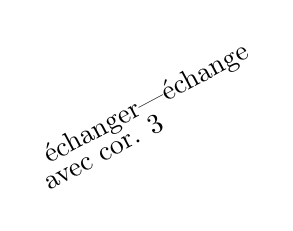
\begin{tikzpicture}[x=1cm,y=1cm]
  \node[anchor=base west,rotate=28] at (0,0.24) {\unsure{échanger|échange}};
  \node[anchor=base west,rotate=28] at (0,-0.10) {avec cor. $3$};
\end{tikzpicture}}}\normalmarginpar
% Slanted note in the left margin; no additional question mark follows the 3.

Soit \unsure{en} ef\deleted{\unsure{i}}\inserted{f}et $D$ \deleted{\unsure{une droite}}\inserted{le sous-espace} propre sous $c$ correspondant à une racine primitive $h$.ème de $1$. Alors $\dim D=1$ (prop.\handwritten{30}), et $\handwritten{\unsure{\mathfrak{z}|z}}=\operatorname{Centr}(\handwritten{\mu})$ normalise $D$, d'où un homomorphisme $\handwritten{\mathfrak{z}\to}\operatorname{Aut}(D)=\underline{C}^{\handwritten{*}}$, dont l'image est un sous-groupe fini de $\underline{C}^{\handwritten{*}}$, contenant l'image (isomorphe) de $\handwritten{\mu}$, donc cyclique d'ordre un multiple de $h$. Grâce à Kostant, son ordre est égal à $h$, et on a donc trouvé une rétraction $\handwritten{\mathfrak{z}\to\mu}$, il faut prouver que son noyau est réduit à $1$. Or si $w$ est dans ce noyau, il \deleted{induit} centralise $D$, et q\unsure{ô|ö}mme $D$ est régulière par Kostant,cela implique $w=1$. \unsure{Bn|On} a donc prouvé $\handwritten{\mathfrak{z}}=\handwritten{\mu}$. Reste à prouver que si $n$ est un entier premier à $h$, alors $c^n$ est conjugué de $c$, ce qui résulte également de Kostant.
% Each centralizer glyph combines a typed z-shaped upper part with a handwritten lower loop.

\uline{Corollaire}. Soit $c$ un élément de Coxeter, et $\handwritten{\lambda}$ une valeur propre de $c$, correspondant à un vecteur propre $x$. Pour que $x$ soit régulier, il faut et il suffit que $\handwritten{\lambda}$ soit une racine primitive $h$.ème de $1$.
\reversemarginpar\margin{\handwritten{\figure{
\begin{tikzpicture}[x=1cm,y=1cm]\draw (0.05,0)--(0,-0.15)--(0,-1.05);\end{tikzpicture}}}}\normalmarginpar

La suffisance a déjà été énoncée avec le th. de Kostant. Pour la nécessité, soit $h'\handwritten{\leq}h$ l'ordre de la valeur propre, alors $\unsure{\mathbin{.}}c^{h'}$ centralise $x$, donc, $x$ étant régulier, on a $c^{h'}=1$, donc $h'=h$, cqfd.

\uline{Corollaire}. 
\begin{tikzpicture}[baseline=(live.base),x=1cm,y=1cm]
  \node[anchor=base west,inner sep=0pt] at (0.15,0.39) {\deleted{\unsure{Considérons}}};
  \node[anchor=base west,inner sep=0pt] (live) at (0,0.14) {\inserted{Soit $D$ une}};
  \node[anchor=base west,inner sep=0pt] at (0,-0.12) {\deleted{Soit $D$ une}};
\end{tikzpicture} droite régulières dans $V\mathbin{\text{\textcircled{x}}}\underline{C}$ telle qu'il existe un élé%
% archive sheet number: 1
\scanpage{3}ment de Coxeter\inserted{\handwritten{$c$}} de $W$ qui la normalise. Alors le normalisateur de $\deleted{W}D$ dans $W$ est le groupe engendré par $c$, et il existe une unique élément de Coxeter de $W$ normalisant $D$ et y ayant pour valeur propre une racine \deleted{de}primitive 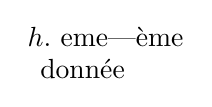
\begin{tikzpicture}[baseline=(given.base)]
\node[inner sep=0pt,anchor=base west] (given) at (0,0) {donnée};
\node[inner sep=0pt,anchor=base west] at (-0.16,0.40) {\inserted{$h$.\ \unsure{eme|ème}}};
\end{tikzpicture} de $1$. Les droites régulières $D$ ayant la propriété précédente (appelées ``droites cycliques'' par Kostant) sont conjuguées sous $W$, leur nombre est égal à $\operatorname{card}(W)/h$.
% The typed h. eme is interlinear, beginning slightly left of donnée; no caret establishes a linear insertion point.

NB Dans l'ensemble des droites cycliques, le groupe $(\underline{Z}/h\underline{Z})^{\handwritten{*}}$ opère\inserted{en commutant à l'action de $W$} librement; deux droites cycliques sont conjuguées sous l'action de ce groupe si et seulement si elles ont même stabilisateur dans $W$.
% archive sheet number: 2

\scanpage{16}
Résumé de quelques résultats de Kostant (sous groupes simples de rang $1$).

$G$ est un groupe semi-simple sur un corps $k$ de car. nulle, $\handwritten{\unsure{\mathfrak{g}|\mathscr{G}}}$ son algèbre de Lie,
\margin{\handwritten{(The principal 3-dimensional subgroup...., Am. Jour. Oct.1959, 3.4, 3.5, 3.6, 1.2, 9.3)}}

\uline{Théorème} 1. \inserted{\handwritten{(i)}} Soient $x,e\handwritten{\in\mathfrak{g}}$,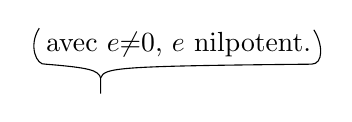
\begin{tikzpicture}[baseline=(attachment)]
\coordinate (attachment) at (0,0);
\node[anchor=base west,inner sep=0pt] (qual) at (-.7,.43) {\inserted{avec $e\handwritten{\ne}0$, $e$ nilpotent.}};
\draw ([xshift=-.08cm,yshift=.05cm]qual.north west) .. controls ([xshift=-.22cm]qual.west) and ([xshift=-.12cm,yshift=-.10cm]qual.south west) .. ([yshift=-.08cm]qual.south west) .. controls (-.15,.23) and (-.03,.20) .. (0,.10) -- (0,-.10);
\draw (0,.10) .. controls (.05,.23) and (.18,.25) .. ([yshift=-.08cm]qual.south east) .. controls ([xshift=.15cm,yshift=-.08cm]qual.south east) and ([xshift=.15cm]qual.east) .. ([xshift=.03cm,yshift=.03cm]qual.north east);
\end{tikzpicture} Pour tout entier $k$, soit $\handwritten{\mathfrak{g}}(k)$ le sous-espace propre de\hspace{1.5em} correspondant à la valeur propre $k$. Donc si $x=\mathop{\mathbb{L}\mathrm{ie}}(i)(1)$, où $i:\underline{G}_m\handwritten{\longrightarrow}G$, les $\handwritten{\mathfrak{g}}(k)$ sont les \deleted{décomposition} composants de $\handwritten{\mathfrak{g}}$ suivant les caractères de $\underline{G}_m$, opérant sur $\handwritten{\mathfrak{g}}$ via $i$ et la représentation adjointe. Les conditions suivantes sont équiva\deleted{\unsure{e}}lentes:

\[
\begin{aligned}
\text{a)}\quad &e\handwritten{\in\mathfrak{g}}(2)\quad\text{i.e.}\quad \handwritten{[}x,e\handwritten{]}=2e,\quad\text{et }\inserted{\text{pour tout entier }k\handwritten{\geq}1,}\\
&\operatorname{ad}(e)^k:\handwritten{\mathfrak{g}}(-k)\handwritten{\longrightarrow\mathfrak{g}}(k)\quad\text{est un isom}\unsure{.}
\end{aligned}
\]

\figure{\begin{tikzpicture}[every node/.style={anchor=base west,inner sep=0pt,font=\scriptsize}]
\node (bmain) at (0,0) {$\text{b)}\quad e\handwritten{\in\mathfrak{g}}(2),\quad\deleted{\unsure{et}}\quad\operatorname{ad}(e):\handwritten{\mathfrak{g}}(0)\handwritten{\longrightarrow\mathfrak{g}}(-2)\quad\text{est surjectif},$};
\node[xshift=.08cm] (addfirst) at (bmain.base east) {\inserted{\handwritten{et $x$ est de la forme}}};
\node (bprime) at (0,-.55) {\handwritten{\deleted{b') Comme b), avec $\operatorname{ad}(e):\mathfrak{g}(0)\to\mathfrak{g}(\unsure{2|-2})$ \uline{\unsure{bijectif}}}}};
\node[xshift=.18cm] (addlast) at (bprime.base east) {\inserted{\handwritten{$f(x_{\unsure{o|0}})$, pour $f:\operatorname{Sl}(2,\unsure{k'|k})\to G$ (\uline{élément de Dynkin}).}}};
% Thin hooked connector, distinct from the heavy b-prime cancellation. Its exact starting attachment is uncertain.
\path (bprime.north west) -- (bprime.north east) coordinate[pos=.60] (hookstart);
\draw ([yshift=.13cm]hookstart) -- ([yshift=.13cm]bprime.north east) .. controls ([xshift=.20cm,yshift=.13cm]bprime.north east) and ([xshift=.22cm,yshift=-.05cm]bprime.south east) .. ([xshift=.12cm,yshift=-.10cm]bprime.south east) -- ([yshift=-.14cm]addlast.south east);
\end{tikzpicture}}

\[
\text{c)}\quad e\handwritten{\in\mathfrak{g}}(2),\quad\text{et }x\handwritten{\in}\operatorname{ad}(e)(\handwritten{\mathfrak{g}}).
\]

\[
\text{c')}\quad e\handwritten{\in\mathfrak{g}}(2),\quad\text{et }x\handwritten{\in}\operatorname{ad}(e)(\handwritten{\mathfrak{g}}(-2)).
\]

d) Il existe un homomorphisme $f:\operatorname{Sl}(2,k)\handwritten{\longrightarrow}G$ tel que $f^{\handwritten{'}}(e_o)=e,f^{\handwritten{\unsure{''|'}}}(x_o)=x\deleted{y}$ où $(x_o,e_o,f_o)$ est la base de $\operatorname{Lie}\operatorname{Sl}(2,k)$ correspondant à l'épinglage habituel de ce groupe.

C$\overset{\unsure{-}}{\underset{\text{\unsure{e|o}}}{\text{e}}}$s conditions impliquent qu'i\deleted{\unsure{o|b}}l existe un homomorphisme $i:\underline{G}_m\handwritten{\longrightarrow}G$, tel que $\operatorname{Lie}(i)(1)=x$, a fortiori que $x$ est semi-simple. De plus, le $f$ de d) est déterminé de façon unique.

(ii) Pour tout élément nilpotent $e$ de $\handwritten{\mathfrak{g}}$, il existe un \unsure{homomorphisme} $f:\operatorname{Sl}(2,k)\handwritten{\longrightarrow}G$ tel que $f(e_o)=e$, ou ce qui revient au même, tel que $f(u_o)=u$ (où $u=\exp(e)$, $u_o=\exp(e_o)$);\inserted{\handwritten{$f$ est uniquement déterminé \unsure{par} $x=f(x_o)$ i.e., par $i=f\circ i_o$.}} \deleted{e}\handwritten{E}n vertu de (i), il revient au même,\deleted{\unsure{(}}lorsque $e=0$ i\begin{tikzpicture}[baseline=(stop.base)]\node[inner sep=0pt,anchor=base] (stop) at (0,0) {.};\draw[line width=.4pt] (-.08,-.02)--(.06,.25);\end{tikzpicture}e. $u\handwritten{\ne}1$, de dire qu'il existe un $x\handwritten{\in\mathfrak{g}}$ tel que $(x,e)$ satisfasse aux conditions équivalentes de (i), ou encore un homomorphisme $i:\underline{G}_m\handwritten{\longrightarrow}G$ tel que $(\operatorname{Lie}(i)(1),e)$ y satisfasse. Les homomorphismes $f$ en question sont conjugués
% The raised par and Z= have no caret fixing their linear attachment; preserve their physical positions.
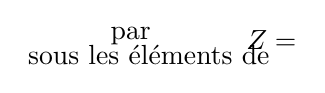
\begin{tikzpicture}[baseline=(cancel.base)]
\node[anchor=base west,inner sep=0pt] (cancel) at (0,0) {\deleted{sous les éléments de}};
\path (cancel.base west) -- (cancel.base east) coordinate[pos=.34] (parpos) coordinate[pos=.90] (zpos);
\node[anchor=base west,inner sep=0pt,yshift=2.1ex] at (parpos) {\inserted{par}};
\node[anchor=base west,inner sep=0pt,yshift=1.3ex] at (zpos) {\inserted{\handwritten{$Z=$}}};
\end{tikzpicture}
$\operatorname{Cent}(\unsure{\begin{tikzpicture}[baseline=(ec.base)]\node[inner sep=0pt,anchor=base] (ec) at (0,0) {$e$};\draw[line width=.45pt] (-.085,.19)--(-.065,.21);\draw[line width=.45pt] (-.015,.27)--(.010,.30);\end{tikzpicture}})=\operatorname{Cent}(u)$ (i.e. pour $e\handwritten{\ne}0$, les $x$ en question, ou encore les $i$ en question, sont conjugués \deleted{sous} par $\operatorname{Cent}(u)$), et lorsque $e\handwritten{\ne}0$, les\deleted{\unsure{morphismes}\quad $g$\quad $\operatorname{int}(g)$} $f$ en question (ou encore les
% archive sheet number: 15
\scanpage{17}
$x$ en question, ou les $i$ en question) forment un \uline{torseur} sous le groupe $\handwritten{Z^+}=$\deleted{$\handwritten{U\unsure{\cap}}\operatorname{Cent}(u)$}\inserted{$\handwritten{Z\cap U}$}, qui est un groupe
% The lower curved enclosure and its descending leader are distinct from the heavy cancellation.
% The endpoint is placed broadly after unipotent, without assigning it to a precise punctuation stroke.
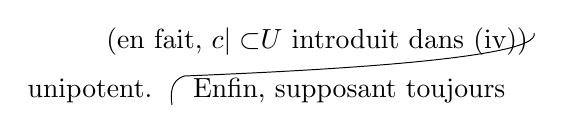
\begin{tikzpicture}[baseline=(unip.base),x=1cm,y=1cm]
\node[anchor=base west,inner sep=0pt] (unip) at (0,0) {unipotent\handwritten{.}};
\node[anchor=base west,inner sep=0pt] at (2.1,0) {Enfin, supposant toujours};
\node[anchor=base west,inner sep=0pt] (cancelnote) at (1.0,.62) {\handwritten{\deleted{(\unsure{en} fait, $\unsure{c|\subset}U$ introduit dans (iv))}}};
\draw[line width=.35pt] ([xshift=2pt,yshift=3pt]cancelnote.east) .. controls ([xshift=5pt,yshift=-7pt]cancelnote.east) and (3.2,.32) .. (2.0,.27) .. controls (1.82,.22) and (1.82,.04) .. (1.84,-.10);
\end{tikzpicture}
% margin note written slanted
\margin{\handwritten{%
% margin note written slanted; the source line positions and split fraction-direct are retained.
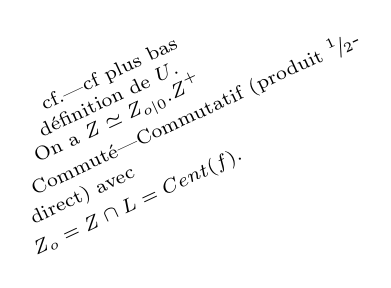
\begin{tikzpicture}[x=.65cm,y=.65cm,every node/.style={anchor=west,inner sep=0pt,font=\scriptsize,rotate=25}]
  \node at (.08,2.85) {\unsure{cf.|cf} plus bas};
  \node at (.02,2.37) {définition de $U$.};
  \node at (-.06,1.84) {On a $Z\simeq Z_{\unsure{o|0}}.Z^+$};
  \node at (-.12,1.22) {\deleted{\unsure{Commuté|Commutatif}} (produit $\unsure{{}^{1}\!/\!_{2}}$-};
  \node at (-.13,.63) {direct) avec};
  \node at (-.08,.02) {$Z_o=Z\cap L=\operatorname{Cent}(f)$.};
\end{tikzpicture}}}
$e\handwritten{\ne}0$, l'ensemble des $x$ en question est un torseur sous \deleted{$\handwritten{\unsure{\mathfrak{g}|\mathscr{G}}}^{e}=$ (centralisateur de $e$ \deleted{\unsure{dans}} dans $\handwritten{\mathfrak{g}}$)$=\operatorname{Ker}\operatorname{ad}(e)=\operatorname{Lie}\operatorname{Cent}(u)$}\inserted{$\handwritten{\operatorname{Lie}(Z^+)=\mathfrak{g}^{e}\cap\operatorname{Fil}^{1}(\mathfrak{g})}$} (\inserted{\handwritten{torseur}}pour l'addition, i.e. est de la forme $a+\handwritten{\mathfrak{g}}^e$, pour un $a\handwritten{\in\mathfrak{g}}$ convenable)\handwritten{.} \deleted{(et on a $\handwritten{\mathfrak{g}}^{e}\handwritten{\subset\sum}_{k\handwritten{\geq}1}\handwritten{\mathfrak{g}}(k)=\operatorname{Fil}^{1}\handwritten{\mathfrak{g}}$)}

(iii) Soit $x\inserted{\handwritten{\ne0}}$ un élément de Dynkin de $\handwritten{\mathfrak{g}}$, donc associé à un homomorphisme de Dynkin $i:\underline{G}_m\handwritten{\longrightarrow}G$. Alors les éléments\inserted{\handwritten{$e$}} de $\handwritten{\mathfrak{g}}$ tels que $(x,e)$ satisfasse\deleted{nt} aux conditions de (i) forment un ouvert dense\inserted{\handwritten{\deleted{$\unsure{\mathfrak{g}(2)^*|\ne0}$}}} de $\handwritten{\mathfrak{g}}(2)$ (savoir l'ouvert\inserted{\handwritten{$\mathfrak{g}(2)^*$}} des points $e$ tels que $\operatorname{ad}(e):\handwritten{\mathfrak{g}}(0)\handwritten{\to\mathfrak{g}}(2)$ soit surjectif), \begin{tikzpicture}[baseline=(oldqui.base),x=1cm,y=1cm]
\node[anchor=base west,inner sep=0pt] (oldqui) at (0,0) {\deleted{qui}};
\node[anchor=base west,inner sep=0pt] at (.85,0) {est un};
\node[anchor=base west,inner sep=0pt] (newcelui) at (.05,.60) {\inserted{\unsure{%
% A typed hyphen is crossed by a separate bowed pen stroke; it is not a typed plus.
\begin{tikzpicture}[baseline=(celui.base)]
\node[anchor=base west,inner sep=0pt] (celui) at (0,0) {Celui};
\node[anchor=base west,inner sep=0pt] (dash) at (celui.base east) {-};
\node[anchor=base west,inner sep=0pt] (ci) at (dash.base east) {ci};
\draw[line width=.5pt] ([xshift=1pt,yshift=6pt]dash.center) .. controls ([xshift=-3pt,yshift=2pt]dash.center) and ([xshift=-3pt,yshift=-2pt]dash.center) .. ([xshift=1pt,yshift=-6pt]dash.center);
\end{tikzpicture}}}};
% Thin lower curve joins the raised replacement to the baseline after the cancelled word.
\draw[line width=.35pt] ([xshift=3pt,yshift=1pt]newcelui.east) .. controls ([xshift=3pt,yshift=-9pt]newcelui.east) and (1.1,.29) .. (.82,.26) .. controls (.66,.23) and (.66,.0) .. (.66,-.16);
\end{tikzpicture} \deleted{\uline{torseur}}\inserted{\handwritten{espace homogène}} sous\inserted{\handwritten{$L=$}}$\operatorname{Cent}(x)=\operatorname{Cent}(i)$, qui est un groupe réductif.

(iv) Bour tout \deleted{couple $(x,e)$ satisfaisant les conditions de (i),}\inserted{élément de Dynkin $x$ de $\handwritten{\mathfrak{g}}$, $x=\operatorname{Lie}(i)(1)$,} considérons les sous-groupes $P,U,\inserted{L}$ de $G$ définis par les conditions
\[
\operatorname{Lie}P=\handwritten{\sum}_{k\handwritten{\geq}0}\handwritten{\mathfrak{g}}(k)\quad,\quad
\operatorname{Lie}U=\handwritten{\sum}_{k\handwritten{\geq}\deleted{0}1}\handwritten{\mathfrak{g}}(k),\quad
\operatorname{Lie}L=\handwritten{\mathfrak{g}}(0).
\]
Alors $P$ est un sous-groupe parabolique de $G$, $U$ est son radical unipotent, et $L=\operatorname{Cent}(x)=\operatorname{Cent}(i)$ \deleted{\unsure{en|un}} est un sous-groupe de Lévi de $G$. Si $\unsure{u|a}\inserted{=\exp(e)}$ est un élément unipotent de $G$ tel que $(i,u)$ soit un couple de Dynkin (i.e. induit par un $f:\unsure{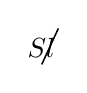
\begin{tikzpicture}[baseline=(sl.base)]
\node[inner sep=0pt] (sl) {$\operatorname{Sl}$};
\draw[line width=.55pt] ([xshift=-5pt,yshift=-6pt]sl.east) -- ([xshift=1pt,yshift=7pt]sl.east);
\end{tikzpicture}}(2,k)\handwritten{\to}G$), $P$ (donc a\unsure{a|u}ssi $U$) est défini en termes de $u$ (i.e; deux $x$ associés au même $u$ donnent le même $P$, cf. (ii)); il en est de même du sous-groupe $H=i(\underline{G}_m).U$ de $G$ (NB $i(\underline{G}_m)$ normalise $U$, et $H$ est un produit semi-direct), et de $i$ mod $U$ i.e. de $\underline{G}_m\handwritten{\longrightarrow}H/U$ induit par $i$. \deleted{\unsure{A}}De plus, l'application
\[
g\handwritten{\longmapsto}\operatorname{ad}(g).x
\]
est un\deleted{e} isomorphisme de $U$ avec $x+\operatorname{Fil}^{1}\handwritten{\mathfrak{g}}\inserted{\handwritten{=x+\operatorname{Lie}U}}$ (où on pose $\operatorname{Fil}^{k}\handwritten{\mathfrak{g}}=\handwritten{\sum}_{j\handwritten{\geq}k}\handwritten{\mathfrak{g}}(j)$), et l'application
\[
g\handwritten{\longmapsto}\operatorname{ad}(g).\handwritten{e}
\]
est une application surjective de $U$ sur $e+\operatorname{Fil}^{\handwritten{3}}(\handwritten{\mathfrak{g}})$, ou de $P$ sur $\handwritten{\mathfrak{g}}(2)^{\handwritten{*}}+\operatorname{Fil}^{\handwritten{3}}(\handwritten{\mathfrak{g}})$, où $\handwritten{\mathfrak{g}}(2)^{\handwritten{*}}$ est l'ouvert de $\handwritten{\mathfrak{g}}(2)$ envisagé dans (iii).
% archive sheet number: 16

\scanpage{18}
\uline{Interprétations en termes de filtrations du foncteur oubli \deleted{sur la catégorie}} des représentations linéaires de dimension finie de $G$. (Il s'agit de
% Typed interlinear addition, with its joined curved enclosure and descending leader.
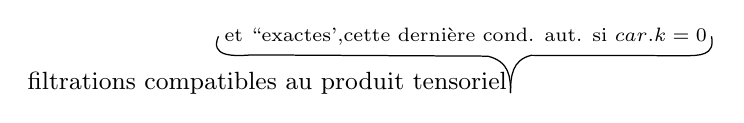
\begin{tikzpicture}[baseline=(body.base),inner sep=0pt,x=1cm,y=1cm]
\node[anchor=base west,font=\small] (body) at (0,0) {filtrations compatibles au produit tensoriel};
\node[anchor=base west,font=\scriptsize] (add) at (2.5,.62) {\inserted{et ``exactes',cette \unsure{dernière} cond. aut. si $\operatorname{car}.k=0$}};
\draw[line width=.45pt] ([xshift=-.07cm]add.west) .. controls ([xshift=-.18cm,yshift=-.14cm]add.south west) and ([xshift=.1cm,yshift=-.14cm]add.south west) .. ([xshift=.35cm,yshift=-.12cm]add.south west) -- ([xshift=-.25cm,yshift=.35cm]body.east) .. controls ([xshift=.03cm,yshift=.28cm]body.east) and ([xshift=.04cm,yshift=.08cm]body.east) .. ([xshift=.04cm,yshift=-.12cm]body.east);
\draw[line width=.45pt] ([xshift=.05cm]add.east) .. controls ([xshift=.1cm,yshift=-.13cm]add.south east) and ([xshift=-.1cm,yshift=-.13cm]add.south east) .. ([xshift=-.3cm,yshift=-.13cm]add.south east) -- ([xshift=.3cm,yshift=.36cm]body.east) .. controls ([xshift=.06cm,yshift=.3cm]body.east) and ([xshift=.04cm,yshift=.1cm]body.east) .. ([xshift=.04cm,yshift=-.12cm]body.east);
\end{tikzpicture}). Supposons fixé une classe
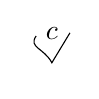
\begin{tikzpicture}[baseline=(base.base),inner sep=0pt]
\node (base) at (0,0) {\phantom{$c$}};
\node at (0,.4) {\inserted{\handwritten{$c$}}};
\draw (-.2,.37) .. controls (-.3,.22) and (-.1,.22) .. (0,.03) -- (.23,.41);
\end{tikzpicture}
de
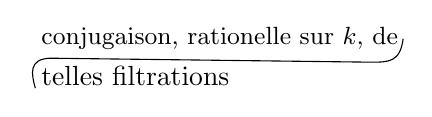
\begin{tikzpicture}[baseline=(base.base),inner sep=0pt,x=1cm,y=1cm]
\node[anchor=base west] (base) at (0,0) {telles filtrations};
\node[anchor=base west,font=\small] (add) at (0,.52) {\inserted{conjugaison, rationelle sur $k$, de}};
\draw ([xshift=.06cm]add.east) .. controls ([xshift=.02cm,yshift=-.15cm]add.south east) and ([xshift=-.12cm,yshift=-.15cm]add.south east) .. ([xshift=-.35cm,yshift=-.15cm]add.south east) -- ([xshift=.12cm,yshift=.23cm]base.west) .. controls ([xshift=-.16cm,yshift=.22cm]base.west) and ([xshift=-.12cm,yshift=.03cm]base.west) .. ([xshift=-.07cm,yshift=-.15cm]base.west);
\end{tikzpicture}
(NB elle n'admet pas nécessairement un représentant rat/$k$); 
% Both o and l contours survive in the second cell; no chronological ordering is assigned.
i\unsure{
\begin{tikzpicture}[baseline=(ol.base),inner sep=0pt]
\node (ol) at (0,0) {o};\node at (0,.01) {l};
\end{tikzpicture}}\deleted{\unsure{n}} revient au même de se donner,\deleted{un} pour le Chevalley $G_o$ associé à $G$, un \deleted{homomorphisme} élément de $\operatorname{Hom}(\underline{G}_m,T_o)/W=M/W$ ($T_o=M\mathbin{\text{\textcircled{x}}}\underline{G}_m$ est le tore maximal type de $G_o$) invariant par le sous-groupe
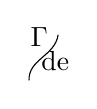
\begin{tikzpicture}[baseline=(base.base),inner sep=0pt]
\node[anchor=base west] (base) at (0,0) {de};
\node at (-.02,.43) {\inserted{\handwritten{$\Gamma$}}};
\draw (-.15,-.12) .. controls (-.16,.15) and (.18,.19) .. (.22,.46);
\end{tikzpicture}
$\operatorname{Auext}G_o=E_o$ image de $\operatorname{Gal}(\handwritten{\bar{k}}/k)$, ou encore un \deleted{homomorphisme $\underline{G}_m\unsure{\to}T$} élément de $M$ qui soit dans la chambre de Weyl de $M\mathbin{\text{\textcircled{x}}}_{\underline{Z}}\underline{R}$ et qui soit stable par $\handwritten{\Gamma}$. On a alors le \unsure{schéma} $\handwritten{\underline{
\begin{tikzpicture}[baseline=-.15ex,x=1ex,y=1ex]\draw[line width=.35pt] (.42,.53) ellipse (.32 and .46);\draw[line width=.35pt] (-.02,-.16)--(.84,1.27);\end{tikzpicture}}_c}$ des filtrations de classe $\handwritten{c}$, qui est un espace homogène sous $G$, de
% The long insertion's enclosure bends down immediately after paraboliques;.
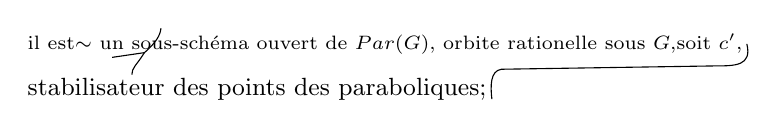
\begin{tikzpicture}[baseline=(base.base),inner sep=0pt,x=1cm,y=1cm]
\node[anchor=base west,font=\small] (base) at (0,0) {stabilisateur des points des paraboliques;};
\node[anchor=base west,font=\scriptsize] (add) at (0,.59) {\inserted{\handwritten{il} est\inserted{\handwritten{$\sim$}} un sous-schéma ouvert de $\uline{Par}(G)$, orbite rationelle sous $G$,\handwritten{soit $c'$,}}};
\draw ([xshift=.05cm]add.east) .. controls ([xshift=.12cm,yshift=-.14cm]add.south east) and ([xshift=-.1cm,yshift=-.14cm]add.south east) .. ([xshift=-.35cm,yshift=-.14cm]add.south east) -- ([xshift=.18cm,yshift=.26cm]base.east) .. controls ([xshift=.04cm,yshift=.24cm]base.east) and ([xshift=.04cm,yshift=.05cm]base.east) .. ([xshift=.06cm,yshift=-.12cm]base.east);
% A second, small curved leader accompanies the raised similarity sign.
\draw (1.08,.49) -- (1.49,.55) .. controls (1.64,.68) and (1.69,.77) .. (1.7,.86);
\draw (1.49,.55) .. controls (1.39,.39) and (1.33,.36) .. (1.33,.27);
\end{tikzpicture}
On peut regarder aussi le schéma $\operatorname{ST}_c$ des homomorphismes $i:\underline{G}_m\handwritten{\to}G$ de classe $c$, qui est donc une orbite rationelle de $G$ opérant sur $\uline{Homgr}(\underline{G}_m,G)$. Il est canoniquement isomorphe au schéma des couples de Lévi $(P,L)$ tels que $P$ soit de classe $c'$. (En d'autres termes, grâce au choix d'un $c$, pour $P$\inserted{\begin{tikzpicture}[baseline=(attach)]
  \node[anchor=west,inner sep=0pt] at (0,.34) {ou encore $\handwritten{\underline{\begin{tikzpicture}[baseline=-.15ex,x=1ex,y=1ex]\draw[line width=.35pt] (.42,.53) ellipse (.32 and .46);\draw[line width=.35pt] (-.02,-.16)--(.84,1.27);\end{tikzpicture}}}$};
  \coordinate (attach) at (-.06,-.15);
  \draw[gray,line width=.25pt] (-.15,-.29) .. controls (-.12,.08) and (.03,.08) .. (.21,.08) -- (2.45,.13) .. controls (2.59,.13) and (2.73,.22) .. (2.78,.43);
  \draw[line width=.5pt] (attach) .. controls (-.06,.16) and (.05,.14) .. (.25,.14) -- (2.84,.14) .. controls (2.98,.14) and (2.99,.23) .. (2.99,.39);
\end{tikzpicture}} de classe $c'$ donné,
il revient au même de se donner un $i:\underline{G}_m\handwritten{\to}P$ de la classe définie par $c$, où un sous-groupe de Lévi de $P$, à $i$ étant associé \unsure{\tikz[baseline=-.45ex]{\fill[rotate=-35] (0,0) ellipse (.35pt and .65pt);}} $\operatorname{Cent}(i)$.\handwritten{)} On a 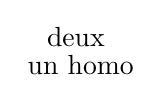
\begin{tikzpicture}[baseline=(old.base),x=1em,y=1em]
\node[anchor=base west,inner sep=0pt] (old) at (0,0) {\deleted{un homo}};
\node[anchor=base west,inner sep=0pt] at (.7,1) {\inserted{deux}};
\end{tikzpicture}morphismesde schémas canoniquement isomorphes
\[
\operatorname{ST}_c\handwritten{\longrightarrow\underline{
\begin{tikzpicture}[baseline=-.15ex,x=1ex,y=1ex]\draw[line width=.35pt] (.42,.53) ellipse (.32 and .46);\draw[line width=.35pt] (-.02,-.16)--(.84,1.27);\end{tikzpicture}}}_c\quad,\quad
(\operatorname{CL})_{c'}\handwritten{\longrightarrow}\operatorname{Par}_{c'}\quad,
\]
le premier en termes de théorie des filtrations d\unsure{%

\begin{tikzpicture}[baseline=(a.base)]
\node[inner sep=0pt] (a) at (0,0) {a};
\node[inner sep=0pt] at (-.015em,.025em) {e};
\end{tikzpicture}} foncteurs fibres, le deuxième \deleted{d}en termes de groupes paraboliques.

Supposons maintenant que $k$ soit de car. nulle (j'ignore dans quelle mesure c'est vraiment nécessaire). On peut alors considérer le Schéma $\operatorname{Dyn}_c$ des homomorphismes $f:\operatorname{Sl}(2,k)\handwritten{\longrightarrow}G$ tels que $fi_o$ soit de classe $c$. Supposons-le
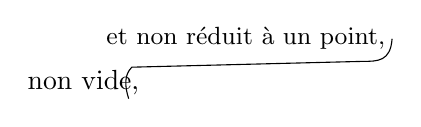
\begin{tikzpicture}[baseline=(base.base),inner sep=0pt,x=1cm,y=1cm]
\node[anchor=base west] (base) at (0,0) {non vide,};
\node[anchor=base west,font=\small] (add) at (1,.56) {\inserted{\handwritten{et non réduit à un point,}}};
\draw ([xshift=.08cm]add.east) .. controls ([xshift=.06cm,yshift=-.14cm]add.south east) and ([xshift=-.1cm,yshift=-.14cm]add.south east) .. ([xshift=-.3cm,yshift=-.14cm]add.south east) -- ([xshift=-.1cm,yshift=.19cm]base.east) .. controls ([xshift=-.2cm,yshift=.09cm]base.east) and ([xshift=-.19cm,yshift=-.05cm]base.east) .. ([xshift=-.14cm,yshift=-.21cm]base.east);
\end{tikzpicture}
i.e. $c$ une classe de
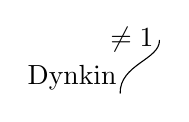
\begin{tikzpicture}[baseline=(base.base),inner sep=0pt]
\node[anchor=base west] (base) at (0,0) {Dynkin};
\node[anchor=base west] (add) at (1.05,.48) {\inserted{\handwritten{$\ne1$}}};
\draw ([xshift=.07cm]add.east) .. controls ([xshift=.08cm,yshift=-.25cm]add.east) and ([xshift=.03cm,yshift=.17cm]base.east) .. ([xshift=.04cm,yshift=-.2cm]base.east);
\end{tikzpicture}.
Alors $\operatorname{Dyn}_c$ est un \deleted{\uline{torseur}}\inserted{\handwritten{espace homogène}} sous $G$
\inserted{\handwritten{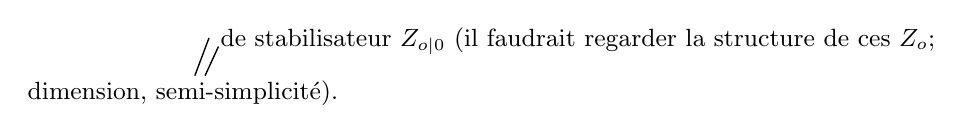
\begin{tikzpicture}[baseline=(attach)]
  \node[anchor=west,inner sep=0pt,font=\small] at (0,.42) {de stabilisateur $Z_{\unsure{o|0}}$ (il faudrait regarder la structure de ces $Z_o$;};
  \node[anchor=west,inner sep=0pt,font=\small] at (-2.45,-.24) {dimension, semi-simplicité).};
  \coordinate (attach) at (-.25,0);
  \draw[line width=.5pt] (-.32,-.02) -- (-.14,.46);
  \draw[line width=.5pt] (-.19,-.02) -- (-.02,.35);
\end{tikzpicture}}}\deleted{(en fait, il est can. is. au torseur $\uline{Isom}(G_1,G)$, où $G_1$ est le groupe quasi-déployé correspondant à $G$).} Soit $\operatorname{Un}_c$ le schéma des éléments
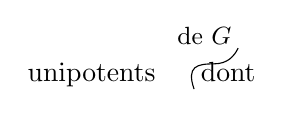
\begin{tikzpicture}[baseline=(base.base),inner sep=0pt,x=1cm,y=1cm]
\node[anchor=base west] (base) at (0,0) {unipotents};
\node[anchor=base west] (tail) at (2.2,0) {dont};
\node[anchor=base west,font=\small] (add) at (1.9,.46) {\inserted{\handwritten{de $G$}}};
\draw (2.12,-.1) .. controls (2.02,.19) and (2.16,.22) .. (2.37,.22) .. controls (2.55,.22) and (2.63,.32) .. (2.68,.42);
\end{tikzpicture}
la classe corresponde à \deleted{celle de} $c$ par la correspondance
% archive sheet number: 17
\scanpage{19}
de Kostant. On a donc \unsure{
\begin{tikzpicture}[baseline=(ud.base)]\node[inner sep=0pt,anchor=base] (ud) at (0,0) {u};\node[inner sep=0pt,anchor=base] at (.025,0) {d};\end{tikzpicture}}\unsure{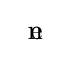
\begin{tikzpicture}[baseline=(ne.base)]\node[inner sep=0pt,anchor=base] (ne) at (0,0) {n};\node[inner sep=0pt,anchor=base] at (.015,0) {e};\end{tikzpicture}}s morphismes $f\handwritten{\unsure{\mathrel{\mapstochar\relbar}|\mapsto}}f\handwritten{\circ}i_o$ et $f\handwritten{\mapsto}f(u_o)$ de $\operatorname{Dyn}_c$ dans $\operatorname{ST}_c$ resp. $\operatorname{Un}_c$. D'autre part, Deligne nous fournit $\operatorname{Un}_c\handwritten{\to\underline{
\begin{tikzpicture}[baseline=-.15ex,x=1ex,y=1ex]\draw[line width=.35pt] (.42,.53) ellipse (.32 and .46);\draw[line width=.35pt] (-.02,-.16)--(.84,1.27);\end{tikzpicture}}}_c$, et celui-ci peut aussi être défini par la commutativité du diagramme \handwritten{d'esp. homogènes}
% The two first cells of the overprinted word preserve u/d and n/e contours; order is uncertain.
\diagram{\begin{tikzpicture}
\node[anchor=north west,inner sep=0pt] at (0,0) {\begin{tikzcd}[ampersand replacement=\&,column sep=large,row sep=large]
\operatorname{ST}_c\handwritten{\simeq}(\operatorname{CL})_{c'} \handwritten{\arrow[d]}
\arrow[d,draw=gray!45,-,to path={([xshift=-.25ex,yshift=.45ex]\tikztotarget.north) .. controls +(0,-.65ex) and +(0,-.65ex) .. ([xshift=.25ex,yshift=.45ex]\tikztotarget.north)}]
\arrow[d,phantom,"{\unsure{}}" description,near end]
\& \operatorname{Dyn}_c \handwritten{\arrow[l]} \handwritten{\arrow[d]} \\
\handwritten{\underline{\begin{tikzpicture}[baseline=-.15ex,x=1ex,y=1ex]\draw[line width=.35pt] (.42,.53) ellipse (.32 and .46);\draw[line width=.35pt] (-.02,-.16)--(.84,1.27);\end{tikzpicture}}}_c\handwritten{\simeq}\operatorname{Par}_{c'} \& \operatorname{Un}_c\quad\text{.} \handwritten{\arrow[l]}
\end{tikzcd}};
\node[anchor=north west,inner sep=0pt] at (7.3,0) {\handwritten{\begin{tikzcd}[ampersand replacement=\&,column sep=small,row sep=small]
L \arrow[d] \& \unsure{\text{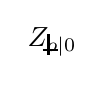
\begin{tikzpicture}[baseline=(zo.base)]\node[inner sep=0pt] (zo) at (0,0) {$Z_{\unsure{o|0}}$};\draw[line width=1.1pt] (-.04,.10) -- (-.04,-.17);\draw[line width=.8pt] (-.12,-.10) -- (.07,-.10);\end{tikzpicture}}} \arrow[l] \arrow[d] \\
P \& \unsure{\mathfrak{z}|z|Z}(\unsure{\mathord{\cdot}}e) \arrow[l]
\end{tikzcd}}};
\end{tikzpicture}}
% The extra strokes on the small square's Z are retained graphically; their predecessor and order are not established.

Pour qu'il existe un point rationnel de \deleted{$\operatorname{Dyn}_c$, ou ce qui revient au même} $\handwritten{\underline{
\begin{tikzpicture}[baseline=-.15ex,x=1ex,y=1ex]\draw[line width=.35pt] (.42,.53) ellipse (.32 and .46);\draw[line width=.35pt] (-.02,-.16)--(.84,1.27);\end{tikzpicture}}}_c\handwritten{\simeq}\operatorname{Par}_{c'}$, il faut (et suffit) qu'il en existe un de $\operatorname{Dy}\unsure{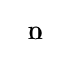
\begin{tikzpicture}[baseline=(n.base)]\node[inner sep=0pt] (n) {$\mathrm n$};\node[inner sep=0pt] at ([xshift=.02em,yshift=-.02ex]n.center) {$\mathrm o$};\end{tikzpicture}}_c$ \deleted{i.e. que $G$ soit quasi-déployé\unsure{;}}\inserted{\handwritten{(i.e.,, si $Z_o=e$, que $G$ est quasi-déployé)}}: en effet, $P$ étant choisi, \deleted{\unsure{les|des} $i$}\begin{tikzpicture}[baseline=-.1ex]\draw[line width=.3pt](0,0)--(.48em,.8ex);\draw[line width=.3pt](0,.8ex)--(.48em,0);\end{tikzpicture} on peut en choisir un \deleted{point rationnel}\begin{tikzpicture}[baseline=-.1ex]\draw[line width=.3pt](0,0)--(.48em,.8ex);\draw[line width=.3pt](0,.8ex)--(.48em,0);\end{tikzpicture} sous-groupe de Lévi
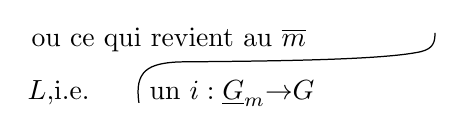
\begin{tikzpicture}[baseline=(levi.base)]
\node[anchor=base west,inner sep=0pt] (levi) at (0,0) {$L$,\deleted{i.e}.};
\node[anchor=base west,inner sep=0pt] at (1.55,0) {un $i:\underline{G}_m\handwritten{\to}G$};
\node[anchor=base west,inner sep=0pt] at (.05,.68) {\inserted{\handwritten{ou ce qui revient au $\overline{m}$}}};
\draw[line width=.45pt] (1.42,-.04) .. controls (1.36,.37) and (1.54,.46) .. (1.92,.48) .. controls (3.00,.49) and (4.50,.50) .. (5.00,.61) .. controls (5.16,.65) and (5.18,.73) .. (5.18,.85);
\end{tikzpicture}
dans la classe $c$,définissant $P$, et alors les $u=\exp(e)$ qui \deleted{\unsure{aue|aux}} s'adaptent à $i$ forment un ouvert dense de $\handwritten{\unsure{\mathfrak{g}|\mathscr{G}}(\unsure{2|\underline{2}})}$, qui \deleted{est donc non vide} a donc un point rationnel. On voit donc que pour certaines classes de paraboliques (qu'on pourrait appeler les paraboliques de
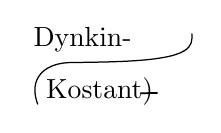
\begin{tikzpicture}[baseline=(kostant.base)]
\node[anchor=base west,inner sep=0pt] (kostant) at (.16,0) {Kostant\unsure{)}};
\draw[line width=.65pt] ([xshift=-.48em,yshift=.4ex]kostant.base east)--++(.62em,.03ex);
\node[anchor=base west,inner sep=0pt] at (0,.65) {\inserted{Dynkin-}};
\draw[line width=.45pt] (.06,-.08) .. controls (-.06,.24) and (.13,.43) .. (.44,.45) .. controls (.90,.46) and (1.68,.45) .. (1.92,.60) .. controls (2.02,.66) and (2.02,.73) .. (2.02,.82);
\end{tikzpicture}
l'existence d'un parabolique de cette classe rationnel sur $k$ implique déjà que $G$ est quasi-déployé. (NB Quand $G$ n'est pas une forme intérieure, il faut faire attention cependant de vérifier d'abord que la classe $c'$ de $P$ provient bien d'un $c$ de Dynkin \uline{invariant par} $\handwritten{\Gamma}$, et il n'est pas clair que cette propriété
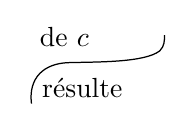
\begin{tikzpicture}[baseline=(resulte.base)]
\node[anchor=base west,inner sep=0pt] (resulte) at (.15,0) {résulte};
\node[anchor=base west,inner sep=0pt] at (.12,.64) {\inserted{de $c$}};
\draw[line width=.45pt] (.02,-.08) .. controls (-.02,.25) and (.18,.43) .. (.49,.44) .. controls (.86,.45) and (1.46,.44) .. (1.65,.59) .. controls (1.71,.65) and (1.71,.72) .. (1.71,.79);
\end{tikzpicture}
du fait que $c'$ est invariant\unsure{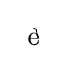
\begin{tikzpicture}[baseline=(endletter.base)]\node[inner sep=0pt,anchor=base] (endletter) at (0,0) {e};\draw[line width=.3pt] ([xshift=.37em,yshift=.82ex]endletter.base west)--++(-.04em,.5ex)--++(-.1em,.12ex);\draw[line width=.25pt] ([xshift=.40em,yshift=.45ex]endletter.base west) .. controls +(.02em,-.25ex) and +(.12em,-.02ex) .. ([xshift=.23em,yshift=.05ex]endletter.base west);\end{tikzpicture}} par $\handwritten{\Gamma}$, faute de savoir si $c\handwritten{\mapsto}c'$ est injectif sur les classes de Dynkin). \handwritten{(}On notera aussi que l'argument donné \unsure{
\begin{tikzpicture}[baseline=(m.base)]\node[inner sep=0pt] (m) {m};\node[inner sep=0pt] at ([xshift=.01em,yshift=-.01ex]m.center) {p};\end{tikzpicture}}arche également sur un anneau semi-local (de car. nulle jusqu'à nouvel ordre).\handwritten{)}
\margin{\handwritten{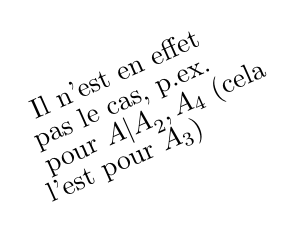
\begin{tikzpicture}[rotate=24,transform shape]
\node[anchor=base west,inner sep=0pt] at (0,0) {Il n'est en effet};
\node[anchor=base west,inner sep=0pt] at (-.12,-.35) {pas le cas, p.ex.};
\node[anchor=base west,inner sep=0pt] at (-.12,-.70) {pour $\unsure{A|\mathbb{A}}_2,A_4$ (cela};
\node[anchor=base west,inner sep=0pt] at (-.24,-1.05) {l'est pour $A_3$)};
\end{tikzpicture}}}
% margin note written slanted, rising to the right
Ceci montre l'intérêt, pour \unsure{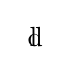
\begin{tikzpicture}[baseline=(ld.base)]\node[inner sep=0pt,anchor=base] (ld) at (0,0) {l};\node[inner sep=0pt,anchor=base] at (.025,0) {d};\end{tikzpicture}}es questions arithmétiques, de déterminer exactement les
\begin{tikzpicture}[baseline=(sous.base)]
\node[anchor=base west,inner sep=0pt] (sous) at (.17,0) {sous-groupes};
\node[anchor=base west,inner sep=0pt] at (0,.63) {\inserted{classes\,\raisebox{.45ex}{\handwritten{de}}}};
\draw[line width=.45pt] (.03,-.07) .. controls (-.02,.20) and (.22,.42) .. (.58,.44) .. controls (1.10,.47) and (1.54,.36) .. (1.96,.58) .. controls (2.04,.64) and (2.06,.71) .. (2.07,.78);
\end{tikzpicture}
parab\handwritten{\unsure{\begin{tikzpicture}[baseline=-.2ex]\draw[line width=.7pt] (0,-.025) -- (.25,.045);\draw[line width=.2pt,gray!50] (.025,.07)--(.25,.17);\end{tikzpicture}}}oliques de Dynkin-Kostant des divers groupes simples, et de voir si: leur stabilisateur dans $\operatorname{Autext}(G_o)$ est le même que celui des $c$ de Dynkin correspondants, et pas str. plus grand.
% The d/l overprint is retained without assigning a chronological order.
% The diagonal joining stroke in paraboliques is drawn, not silently treated as a lexical hyphen.

On notera cependant que si une filtration du foncteur \deleted{fib} oubli peut être définie par un élément unipotent, la classe de conjugaison de ce der%
% Source has a line-end hyphen after der; the word continues beyond this scan.
% archive sheet number: 18
\scanpage{20}nier (ou, ce qui revient au même, $c$) est bien déterminée. Les unipotents qui définissent ladite filtration, en termes d'un $i$ qui la définit, sont
% Typed interlinear addition and its connected handwritten curved leader.
\begin{tikzpicture}[baseline=(de.base),x=1em,y=1ex]
\node[anchor=base west,inner sep=0pt] (de) at (0,0) {de};
\node[anchor=base west,inner sep=0pt] at (0,2.05) {\inserted{ceux}};
\draw[line width=.45pt] (-.45,-.10) .. controls (-.28,.75) and (.08,1.65) .. (.78,1.62) .. controls (1.32,1.55) and (2.12,1.34) .. (2.20,2.16);
\end{tikzpicture}
la forme $\exp(e)$, où $e$ parcourt $\handwritten{\unsure{\mathfrak{g}|\mathscr{G}}}(2)^{\handwritten{*}}+\operatorname{Fil}^{\handwritten{3}}(\handwritten{\mathfrak{g}})$. Ils forment une classe de conjugaison d'éléments de $U$ \uline{par} $P$ (NB mais pas par $U$), les classes de conjugaison \uline{par} $U$ s'identifiant aux ensembles de la forme $(\exp(e)\handwritten{\mid}e\handwritten{\in}a+\operatorname{Fil}^{\handwritten{3}}(\handwritten{\mathfrak{g}}\unsure{.|,}))$, où $a\handwritten{\in\mathfrak{g}}(2)^{\handwritten{*}}$ est un élément quelconque.\deleted{de}

\uline{Cas principal}. Pour qu'on ait\hspace{1.5em}$(1)=0$, il faut et suffit que \deleted{l'homomor} la classe d'homomorphismes $f:\operatorname{Sl}(2,k)\hspace{1.5em}G$ envisagée soit ``princi%
% Each of these two cells has p and a contours; their chronological order is unresolved.
\unsure{\begin{tikzpicture}[baseline=(pa.base),x=1em,y=1ex]
\node[anchor=base west,inner sep=0pt] (pa) at (0,0) {p};
\node[anchor=base west,inner sep=0pt] at (.02,.10) {a};
\node[anchor=base west,inner sep=0pt] at (.56,0) {a};
\node[anchor=base west,inner sep=0pt] at (.56,-.05) {p};
\end{tikzpicture}}%
le'' au sens de Dynkin-Kostant. Alors le parabolique associé $P$ est un Borel
% slanted
\reversemarginpar
\margin{\handwritten{\begin{tikzpicture}[x=1em,y=1ex,scale=.61,transform shape]
  \begin{scope}[rotate=18]
    \node[anchor=base west,inner sep=0pt] at (0,0) {\uline{ex}};
    \node[anchor=base west,inner sep=0pt] at (2.4,.10) {Cas $A_2,A_4$};
    \node[anchor=base west,inner sep=0pt] at (-.10,-2.40) {les paraboliques associés};
    \node[anchor=base west,inner sep=0pt] at (-.15,-4.80) {aux \unsure{unipotents}};
    \node[anchor=base west,inner sep=0pt] at (-.15,-7.20) {``sous-réguliers'' sont};
    \node[anchor=base west,inner sep=0pt] at (-.15,-9.60) {des \unsure{borels|Borels} !};
  \end{scope}
\end{tikzpicture}}}
\normalmarginpar
(la réciproque n'étant pas vraie \deleted{sans doute}, cf table de Dynkin), et le groupe $Z_o$ est le groupe unité (i.e. $\operatorname{Dyn}_c$ est un torseur sous $G$),
% Serifed l contour plus an unresolved two-loop overprint; no order of impressions is assigned.
\unsure{\begin{tikzpicture}[baseline=(base.base),x=1em,y=1ex]
  \node[anchor=base,inner sep=0pt] (base) at (0,0) {l};
  \draw[line width=.28pt] (.10,1.35) .. controls (-.30,1.62) and (-.29,.91) .. (-.03,.70)
    .. controls (.34,.52) and (.36,.18) .. (.13,.03)
    .. controls (-.10,-.02) and (-.31,.23) .. (-.18,.48);
  \draw[line width=.22pt] (-.08,-.28)--(-.08,.05);
  \draw[line width=.22pt] (.12,-.30)--(.12,.05);
  \draw[line width=.22pt] (.12,1.35)--(.30,1.29);
  \fill (.20,1.65) circle[radius=.025em];
\end{tikzpicture}}a réciproque n'étant pas vraie sans doute.
% archive sheet number: 19

\scanpage{22}
\hfill\handwritten{\unsure{Massy} 22. 10. 1969}\\

Dear Kostant,\\

I read again through your papers in the \unsure{Maer.|Amer.} Journ. on \handwritten{``}\deleted{t}\handwritten{T}he principal three-dimensional subgroup ...\handwritten{''} and \handwritten{``}Lie group representations on polynom\begin{tikzpicture}[baseline=(letters.base),x=1em,y=1em]
\node[inner sep=0pt] (letters) at (0,0) {ai};
\handwritten{\draw[line width=.6pt] (-.30,.72) .. controls (-.04,.55) and (-.16,-.55) .. (.19,-.48) .. controls (.34,-.46) and (.44,-.22) .. (.42,-.16);}
\end{tikzpicture}l rings\handwritten{''}, prompted by some nice work of Brieskorn on Klein singularities. I very much appreciate this work of yours, and would appreciate getting reprints of any later work you may have available. As I already felt when your work appea\unsure{\begin{tikzpicture}[baseline=(letters.base),x=1em,y=1em]
\node[inner sep=0pt] (letters) at (0,0) {r};
\handwritten{\draw[line width=.5pt] (-.04,.36)--(.15,.93);
\draw[line width=.5pt] (.02,.06)--(.27,-.19);}
\end{tikzpicture}}ed, it cries for careful reconsideration in the framework of \deleted{\unsure{a|A}}\handwritten{A}lg. Geometry, and suggests number of interesting problems. I wonder if you know the answer to some of them. For instance, I feel it would be of interest to classify (for a given complex simple adjoint Lie group, say) quadr\deleted{\unsure{a|u}}uples $(\mathrm{T},\mathrm{B},\mathrm{T}',\mathrm{B}')$, where $\mathrm{T}$ and $\mathrm{T}'$ are maximal tori ``in apposition\handwritten{''} (in your terminology), and $\mathrm{B}$ and $\mathrm{B}'$ Borel subgroups of $\mathrm{G}$ containing $\mathrm{T}$ resp. $\mathrm{T}'$. The number of conjugacy classes of such animals is equal to $\operatorname{card}(\mathrm{W})^{2}/\mathrm{hz}\handwritten{\begin{tikzpicture}[baseline=-.15ex,x=1ex,y=1ex]\draw[line width=.35pt] (.42,.53) ellipse (.32 and .46);\draw[line width=.35pt] (-.02,-.16)--(.84,1.27);\end{tikzpicture}}(\mathrm{h})$, where $\deleted{\unsure{\mathrm{H}|\mathrm{W}}}\handwritten{W}$ is the Weyl group, $\mathrm{h}$ the Coxeter number, $\mathrm{z}$ the order of the \begin{tikzpicture}[baseline=(center.base),x=1em,y=1em]
\node[inner sep=0pt] (center) at (0,0) {center};
\node[inner sep=0pt] at (1.84,0) {,};
\node[inner sep=0pt] at (1.50,1.08) {\inserted{\handwritten{of $\widetilde{G}$}}};
\handwritten{\draw[line width=.35pt] (1.48,-.57) .. controls (1.08,-.30) and (1.56,.34) .. (2.10,.61) .. controls (2.66,.85) and (3.33,.60) .. (3.47,1.12);}
\end{tikzpicture} and $\handwritten{\begin{tikzpicture}[baseline=-.15ex,x=1ex,y=1ex]\draw[line width=.35pt] (.42,.53) ellipse (.32 and .46);\draw[line width=.35pt] (-.02,-.16)--(.84,1.27);\end{tikzpicture}}(\mathrm{h})=\operatorname{card}(\underline{\mathrm{Z}}/\mathrm{h}\underline{\mathrm{Z}})^{\handwritten{*}}$ is the Euler indicatrix; if you want to classify such data with moreover a\deleted{n} \begin{tikzpicture}[baseline=(element.base),x=1em,y=1em]
\node[inner sep=0pt,anchor=base west] (element) at (0,0) {element};
\node[inner sep=0pt,anchor=base west] at (-.05,1.05) {\inserted{generating}};
\handwritten{\draw[line width=.35pt] (-.20,-.26) .. controls (-.40,.20) and (-.04,.65) .. (.46,.68) .. controls (2.42,.68) and (4.40,.53) .. (4.65,1.16);}
\end{tikzpicture} (principal regular in your terminology) given for the finite group of order $\mathrm{h}$ $\mathrm{T}\handwritten{\cap}\mathrm{N}(\mathrm{T}')$, then we get $\operatorname{card}(\mathrm{W})^{\handwritten{2}}/\mathrm{hz}$ choices. One of the reasons I think this question is interesting is that the stablity subgroup in $\mathrm{G}$ of such a quadruple is $\mathrm{T}\handwritten{\cap}\mathrm{T}'=\mathrm{e}$,\handwritten{\textsuperscript{*}} hence such a structure makes $\mathrm{G}$ entirely ``rigid'' up to exterior automorphisms. Among the first questions one may wish to ask in this direction are the following: is it true that for some, or for all, such quadruples, $\mathrm{B}$ and $\mathrm{B}'$ are ``in general position'' i.e. $\mathrm{B}\handwritten{\cap}\mathrm{B}'$ is a torus (necessarily maximal), so that $\mathrm{B}$ and $\mathrm{B}'$ are ``opposite'' to each other with respect to the latter ? Is there in any sense a \uline{distinguished} conjugacy class of such quadruples (which should then be, of course, invariant by action of exterior automorphisms) ? What are the groups of automorph\unsure{\begin{tikzpicture}[baseline=(letters.base),x=1em,y=1em]
\node[inner sep=0pt] (letters) at (0,0) {k};
\node[inner sep=0pt] at (.08,0) {i};
\end{tikzpicture}}sms of such quadr\deleted{a}uples (they
\margin{\handwritten{\begin{tikzpicture}[x=1cm,y=1cm,every node/.style={inner sep=0pt,anchor=base west,font=\scriptsize}]
\node at (0,0) {* NB:};
\node at (1.23,0) {$N(T)\cap N(T')$};
\node at (3.20,-.02) {is an ext\unsure{e|a}n\unsure{s}ion of};
\node at (6.46,0) {$(\mathbb{Z}/h\mathbb{Z})^{*}$};
\node at (8.20,-.06) {by};
\node at (8.97,-.02) {$\mathbb{Z}/h\unsure{Z|\mathbb{Z}}$};
\node at (10.04,-.02) {$\times$};
\draw[line width=.2pt] (10.13,.36)--(10.13,.25) (10.13,.19)--(10.13,.12) (10.13,-.08)--(10.13,-.16) (10.13,-.22)--(10.13,-.30);
\node at (10.44,.02) {$Z$};
\node at (10.76,-.03) {$\deleted{\unsure{(G)|(\widetilde{G})}}$};
\node at (11.54,-.12) {,};
\draw[line width=.35pt] (10.57,-.06)--(10.48,-.27);
\node at (9.79,-.49) {center of $\widetilde{G}$};
\node[rotate=-3] at (11.92,-.02) {hen\unsure{ce} of ord\unsure{er}};
\node[rotate=-3] at (13.23,-.42) {$hz\varphi(h)$};
\end{tikzpicture}}}
% The thin interrupted trace through the multiplication sign is reproduced without a mathematical function; ink versus surface origin remains uncertain.
% Bottom margin note, with a separate lower annotation beneath Z and a lower-right order formula; right-hand rows slant down to the right.
% The two oblique strokes on the r/k cell of appeared and the overlapping k/i impressions in automorphisms do not establish correction chronology.
% The first exponent 2 is definite as a glyph; its faint impression leaves handwriting versus typewriting unresolved.
% The handwritten transposition stroke crosses the original typed ai in polynomail; no replacement letters have been supplied.
% archive sheet number: 21
\scanpage{23}
are isomorphic to subgroups of the group of exterior automorphisms of $\mathrm{G}$) ?

In a different direction, it would \begin{tikzpicture}[baseline=(e.base),x=1em,y=1ex]
  \node[anchor=base east,inner sep=0] (b) at (0,0) {b};
  \node[anchor=base west,inner sep=0] (e) at (0,0) {e};
  \node[anchor=base west,inner sep=0] at (e.base east) {interesting};
  \draw[line width=.20pt] (e.north) -- ++(0,2.30);
  \draw[line width=.35pt] ([yshift=2.30ex]e.north) -- ++(0,.20);
\end{tikzpicture} to know more about the canonical morphism $\underline{\mathrm{g}}\handwritten{\longrightarrow}\underline{\mathrm{h}}/\mathrm{W}$, where $\underline{\mathrm{g}}$ is the Lie algebra of $\mathrm{G}$ and $\underline{\mathrm{h}}$ a Cartan subalgebra, and of the orbits of $\mathrm{G}$ on $\underline{\mathrm{g}}$, and the analoguous morphism of Steinberg $\mathrm{G}\handwritten{\longrightarrow}\mathrm{T}/\mathrm{W}$ and the orbits of $\mathrm{G}$ acting on itself. Do you know for instance exactly how varies the rank (= rang of the tangent map) of this \deleted{applic\unsure{at}i} map ? There are some reasons to believe that \begin{tikzpicture}[baseline=(th.base),x=1em,y=1ex]
\node[anchor=base west,inner sep=0pt] (th) at (0,0) {\deleted{this}};
\node[anchor=base west,inner sep=0pt] at ([xshift=.10em]th.base east) {\texttt{x}};
\end{tikzpicture} for points of unipotent orbits of \begin{tikzpicture}[baseline=(d.base),x=1em,y=1ex]
\node[anchor=base west,inner sep=0pt] (d) at (0,0) {dimension};
\node[anchor=base west,inner sep=0pt] at (5.0,0) {$\mathrm{r}-2$};
\node[anchor=base west,inner sep=0pt] at (4.05,1.6) {$\inserted{\mathrm{n}-}$};
\draw[line width=.45pt] (3.83,1.8) .. controls (3.5,.7) and (4.65,1.0) .. (4.76,.28) -- (4.76,-.65);
\fill (4.57,-.26) circle[radius=.035em];
\end{tikzpicture} (just \begin{tikzpicture}[baseline=(live.base),x=1em,y=1ex]
\node[anchor=base west,inner sep=0pt] at (0,1.05) {\deleted{the next lower after}};
\node[anchor=base west,inner sep=0pt] (live) at (0,0) {\inserted{the next lower after}};
\end{tikzpicture} the maximal dimension $\mathrm{n}-\mathrm{r}$), the rank is $\mathrm{r}-1$ in case all roots have same length (that is the corresponding diagrams $\mathrm{A}_{\unsure{\begin{tikzpicture}[baseline=(r.base),x=1em,y=1ex]\node[inner sep=0pt] at (0,0) {$\scriptstyle\mathrm{n}$};\node[inner sep=0pt] (r) at (.025,.03) {$\scriptstyle\mathrm{r}$};\end{tikzpicture}|\mathbb{r}}},\mathrm{D}_{\unsure{\text{\begin{tikzpicture}[baseline=(dn.base),x=1em,y=1ex]
  \node[anchor=base,inner sep=0] (dn) at (0,0) {$\scriptstyle\mathrm{n}$};
  \node[anchor=base,inner sep=0] at (.07,-.04) {$\scriptstyle\mathrm{r}$};
  \draw[line width=.25pt] (.16,-.13) -- (.23,-.42);
\end{tikzpicture}}|\mathbb{r}}},\mathrm{E}_{\handwritten{6}},\mathrm{E}_{\handwritten{7}},\mathrm{E}_{\handwritten{8}}$ are those corresponding to Klein singularities), and $\handwritten{<}\mathrm{r}-1$ in \begin{tikzpicture}[baseline=(other.base),x=1em,y=1ex]
\node[anchor=base west,inner sep=0pt] (other) at (.3,0) {other};
\node[anchor=base west,inner sep=0pt] at (.10,1.55) {\inserted{\handwritten{all}}};
\draw[line width=.3pt] (0,-.1) .. controls (.25,1.15) and (1.62,.68) .. (1.8,1.4);
\end{tikzpicture} cases; in the first case, I would expect that there is just one orbit as stated, by the way, and maybe this property will be caracteristic of the ``homogene\deleted{a}ous'' case when all roots have same length. Also, what can be said of the dim\begin{tikzpicture}[baseline=(de.base),x=1em,y=1ex]
\node[anchor=base,inner sep=0pt] (de) at (0,0) {e};
\node[anchor=base,inner sep=0pt] at (.035,.62) {\unsure{o|e}};
\draw[line width=.25pt] (-.16,-.14)--(-.20,-.50);
\draw[line width=.25pt] (.13,-.12)--(.12,-.43);
\draw[line width=.25pt] (.12,.90)--(.26,.58);
\end{tikzpicture}nsion of the set of all Borel subgroups containing a given element $\mathrm{g}\handwritten{\in}\mathrm{G}$, resp. whose Lie algebra contains a given element $\mathrm{x}\handwritten{\in}\underline{\mathrm{g}}$ ? If $2\mathrm{N}=\mathrm{n}-\mathrm{r}$ is the number of roots and if the dimension of the orbit of the given element is $2\mathrm{N}-2\mathrm{i}$, I would expect the dimension of the previous variety to be equal to $\mathrm{i}$; the inequality $\handwritten{\leqslant}\mathrm{i}$ would imply, by generalizing a depth argument of Br\unsure{\begin{tikzpicture}[baseline=(i.base),x=1em,y=1ex]\node[inner sep=0pt] at (0,0) {e};\node[inner sep=0pt] (i) at (-.025,.025) {i};\end{tikzpicture}}\unsure{\begin{tikzpicture}[baseline=(e.base),x=1em,y=1ex]\node[inner sep=0pt] at (0,0) {i};\node[inner sep=0pt] (e) at (.025,.025) {e};\end{tikzpicture}}skorn, that the singularities of the fibers of your map $\underline{\mathrm{g}}\handwritten{\longrightarrow}\underline{\mathrm{h}}/\text{\begin{tikzpicture}[baseline=(ww.base),x=1em,y=1ex]
\node[anchor=base,inner sep=0pt] (ww) at (0,0) {$\mathrm{W}$};
\node[inner sep=0pt] at (.20,-.48) {\unsure{\begin{tikzpicture}[x=1em,y=1ex]\fill (0,0) circle (.20pt);\end{tikzpicture}}};
\end{tikzpicture}}$ (resp. Steinberg's $\mathrm{G}\handwritten{\longrightarrow}\mathrm{T}/\mathrm{W}$ in case $\mathrm{G}$ is simply connected instead of adjoint) are ``rational'', i.e. i\unsure{\begin{tikzpicture}[baseline=(f.base),x=1em,y=1ex]\node[inner sep=0pt] at (0,0) {s};\node[inner sep=0pt] (f) at (0,.025) {f};\end{tikzpicture}} $\mathrm{F}$ is such a fiber and $\mathrm{F}'\overset{\mathrm{f}}{\handwritten{\longrightarrow}}\mathrm{F}$ a resolution of singularities of $\mathrm{F}$, t\unsure{\begin{tikzpicture}[baseline=(h.base),x=1em,y=1ex]\node[inner sep=0pt] at (0,0) {e};\node[inner sep=0pt] (h) at (0,.015) {h};\end{tikzpicture}}\unsure{\begin{tikzpicture}[baseline=(e.base),x=1em,y=1ex]\node[inner sep=0pt] at (0,0) {h};\node[inner sep=0pt] (e) at (0,.015) {e};\end{tikzpicture}}n $\mathrm{R}^{\mathrm{i}}\mathrm{f}_{\handwritten{*}}(\text{\begin{tikzpicture}[baseline=(oo.base),x=1em,y=1ex]
  \node[anchor=base,inner sep=0] (oo) at (0,0) {$\underline{\mathrm{O}}$};
  \node[anchor=base west,inner sep=0] at (.36,-1.02) {$\scriptstyle\mathrm{F}'$};
  \node[anchor=base west,inner sep=0] at (.36,.37) {$\scriptstyle\deleted{\unsure{\mathrm{t}|*}}$};
\end{tikzpicture}})=0$ for $\mathrm{i}\handwritten{>}0$. Maybe the ans\unsure{\begin{tikzpicture}[baseline=(w.base),x=1em,y=1ex]\node[inner sep=0pt] (w) at (0,0) {w};\draw[line width=.35pt] (-.27,.63) -- (-.25,-.38) .. controls (0,-.57) and (.23,-.43) .. (.25,-.30) -- (.25,.58);\end{tikzpicture}|u}\begin{tikzpicture}[baseline=(e.base),x=1em,y=1ex]\node[inner sep=0pt] (e) at (0,0) {e};\draw[line width=.35pt] (-.22,.02) -- (-.22,1.10);\end{tikzpicture}r \deleted{\unsure{ot|to}}\handwritten{to} most of the questions I am asking are well known and I am just ignorant; for some of them, it would indeed be scandalous that the experts do not know the answer ! In any case, I would be grateful for any comment you would have on any of my questions.

\figure{\begin{tikzpicture}[x=1cm,y=1cm]
\node[anchor=base west,inner sep=0pt] at (0,0) {Sincerely yours};
\node[anchor=base west,inner sep=0pt] at (7.0,-.55) {\handwritten{A\,G\unsure{rothendieck}}};
\fill (7.93,-.32) circle[radius=.012cm];
\node[inner sep=0pt] at (8.48,-1.85) {\unsure{\begin{tikzpicture}[x=1cm,y=1cm]
\fill (0,.53) circle[radius=.008cm];
\draw[line width=.25pt] (0,.48)--(0,.41);
\draw[line width=.25pt] (0,.38)--(0,.29);
\draw[line width=.25pt] (-.005,.25)--(-.005,.18);
\draw[line width=.25pt] (0,.16)--(-.005,.07);
\draw[line width=.25pt] (-.005,.05)--(-.005,-.02);
\end{tikzpicture}}};
\end{tikzpicture}}
% The raised line above the e in beinteresting has no assigned textual function.
% Raised n- is definite; typewritten versus pen medium remains uncertain. Its leader and the separate low point are drawn.
% Mixed typewriter impressions are overlaid without assigning an unattested strike order.
% A detached point above the early signature strokes is retained without assigning punctuation.
% The separate interrupted bottom trace is drawn; ink versus surface origin and function remain uncertain.
% archive sheet number: 22

% The extra x following cancelled this is a cancellation impression, not a live word.
% Dimension retains two lower projections and an upper internal diagonal without an inferred predecessor.
% The small isolated point below the later W is drawn with origin/function uncertainty; it is not assigned as punctuation or an index.

\scanpage{28}
\mspage{\handwritten{\unsure{2|7}2}}
% archive sheet number: 27 (inverted at the upper right)
% Source image 1683 x 2140. The whole-sheet cancellation is drawn at the end,
% using anchors in the text; deletion wrappers also record its textual state.
\noindent\begin{tikzpicture}[remember picture,overlay]
\coordinate (p28r1top) at (0,0);
\end{tikzpicture}%
\deleted{un morphisme de topos $\mathrm{u}:\mathrm{E}\handwritten{\longrightarrow}\mathrm{E}'$, et ce dernier sera ``unique à isomorphisme unique près'' en termes de la donnée $\mathrm{u}^{\handwritten{*}}$ resp. $\begin{tikzpicture}[baseline=(p28openingus.base),x=1em,y=1ex]
\node[inner sep=0pt] (p28openingus) at (0,0) {$\mathrm{u}_{\handwritten{*}}$};
\node[inner sep=0pt] at (.61,1.25) {\unsure{\begin{tikzpicture}[x=1em,y=1ex]\draw[gray,line width=.25pt] (0,0)--(.015,.35);\end{tikzpicture}}};
\end{tikzpicture}$, en un sens assez clair, et qui sera d'ailleurs entièrement explicité plus bas \handwritten{(\deleted{\unsure{2|3}}3.2.1)}\unsure{.}}

\deleted{\deleted{2}\handwritten{3}.1.2. Si $\mathrm{u}:\mathrm{E}\handwritten{\longrightarrow}\mathrm{E}'$ est un morphisme de topos, il résulte des propriétés des foncteurs adjoints
\mbox{\begin{tikzpicture}[baseline=(p28r1que.base),x=1em,y=1em]
\node[anchor=base west,inner sep=0pt] (p28r1que) at (0,0) {que};
\node[anchor=base west,inner sep=0pt] at (-.6,1.15) {\inserted{\handwritten{(I 2.11)}}};
\draw[line width=.35pt] (-.25,-.25) .. controls (-.4,.5) and (.1,.75) .. (1.5,.82) .. controls (3.6,.9) and (5.4,.6) .. (5.6,1.02) .. controls (5.8,1.25) and (5.5,1.35) .. (5.35,1.3);
\end{tikzpicture}}
le foncteur image directe $\mathrm{u}_{\handwritten{*}}:\mathrm{E}\handwritten{\longrightarrow}\mathrm{E}'$ commute aux limites projectives, et le foncteur $\mathrm{u}^{\handwritten{*}}:\mathrm{E}'\handwritten{\longrightarrow}\mathrm{E}$ commute aux limites inductives}%
\margin{\handwritten{\deleted{(I \unsure{2.11|4.11})}.}}%
\deleted{ \deleted{\unsure{(2.11)|(I 2.11)}}\handwritten{\mbox{\begin{tikzpicture}[baseline=(p28r1star.base),x=1em,y=1em]
\node[inner sep=0pt] (p28r1star) at (0,0) {$(\phantom{*})$};
\node[inner sep=0pt] at (0,.55) {$*$};
% A definite star; two additional lower prongs have uncertain function.
\node[inner sep=0pt] at (.05,.12) {\unsure{\begin{tikzpicture}[x=1em,y=1em]
\draw[line width=.4pt] (-.12,.3) .. controls (-.2,.15) and (-.2,.04) .. (-.12,0);
\draw[line width=.4pt] (.03,.3) .. controls (.02,.16) and (.07,.06) .. (.08,0);
\end{tikzpicture}}};
\end{tikzpicture}}}.Comme on suppose de plus que ce dernier
\mbox{\begin{tikzpicture}[baseline=(p28r1commute.base),x=1em,y=1em]
\node[anchor=base west,inner sep=0pt] (p28r1commute) at (0,0) {commute};
\node[anchor=base west,inner sep=0pt] at (-3.4,1.2) {\inserted{\handwritten{est ex\unsure{.|a}ct à gauche i.e.}}};
\draw[line width=.35pt] (-.3,-.25) .. controls (-.6,.5) and (-.1,.8) .. (1.15,.9) .. controls (4.1,1.15) and (8.7,.95) .. (9.5,1.1) .. controls (9.9,1.16) and (10,1.35) .. (9.92,1.48);
% Detached point above the right end of the leader; function uncertain.
\node[inner sep=0pt] at (9.72,1.7) {\unsure{\begin{tikzpicture}\fill (0,0) circle (.35pt);\end{tikzpicture}}};
\end{tikzpicture}}
aux limites projectives finies, on voit donc en particulier que $\mathrm{u}^{\handwritten{*}}$ \uline{est} \deleted{exac} \uline{exact}.
\mbox{\begin{tikzpicture}[baseline=(p28r1cest.base),x=1em,y=1em]
\node[anchor=base west,inner sep=0pt] (p28r1cest) at (0,0) {\uline{\deleted{C}\handwritten{c}'est \deleted{donc} le foncteur image inverse}};
\node[anchor=base west,inner sep=0pt] at (-.8,1.12) {\inserted{On peut donc dire que}};
\draw[line width=.35pt] (-.35,-.35) .. controls (-.7,.45) and (-.45,.78) .. (.3,.82) .. controls (4.5,.85) and (10.9,.94) .. (12.6,.9) .. controls (13,.9) and (13.1,1.02) .. (13,1.18);
\end{tikzpicture}}
$\mathrm{u}^{\handwritten{\begin{tikzpicture}[x=.1cm,y=.1cm,baseline=0pt]
\draw[line width=.35pt] (0,.9)--(.6,-.6);
\draw[line width=.35pt] (.6,1)--(-.35,-.8);
\draw[line width=.35pt] (-.15,.1)--(1.3,.1);
\fill (.55,-1.0) circle (.11);
\end{tikzpicture}}}$ \deleted{qui}, dans le couple $(\mathrm{u}_{\handwritten{*}},\mathrm{u}^{\handwritten{\begin{tikzpicture}[x=.1cm,y=.1cm,baseline=0pt]
\draw[line width=.35pt] (-.20,1.0)--(.15,.05);
\draw[line width=.35pt] (-.5,0)--(1.1,0);
\draw[line width=.35pt] (.20,-.35)--(.40,-.88);
\fill (-.48,-.65) circle (.12);
\end{tikzpicture}}})$, \uline{qui possède les propriétés d'exactitude les plus remarquables}, \deleted{assurant} Ces propriétés assurent que pour toute espèce de structure algébrique
\mbox{\begin{tikzpicture}[baseline=(p28r1quipeut.base),x=1em,y=1em]
\node[anchor=base west,inner sep=0pt] (p28r1quipeut) at (0,0) {\deleted{qui}\texttt{x}\deleted{peut}};
% The x between the two cancelled words occupies their otherwise blank cell.
\node[anchor=base west,inner sep=0pt] at (0,1.15) {\inserted{\handwritten{$\Sigma$}}};
\draw[line width=.35pt] (-.25,-.35) .. controls (-.5,.3) and (-.1,.65) .. (1,.78) .. controls (2.5,.82) and (3.7,.93) .. (4,1.12) .. controls (4.15,1.22) and (4.1,1.4) .. (4.1,1.45);
% A separate faint short arc below Sigma, distinct from the insertion leader.
\node[inner sep=0pt] at (.45,.91) {\unsure{\begin{tikzpicture}[x=1em,y=1em]
\draw[line width=.2pt,gray] (0,.12) .. controls (.15,-.08) and (.48,-.04) .. (.72,.1);
\end{tikzpicture}}};
\end{tikzpicture}}
dont les données peuvent se décrire en termes de données de flèches entre les ensembles de base et des ensembles déduits de ceux-ci par \mbox{\begin{tikzpicture}[baseline=(p28application.base),x=1em,y=1ex]
\node[anchor=base west,inner sep=0pt] (p28application) at (0,0) {application};
% Two visible light diagonal stretches; ink versus surface origin is unresolved.
\node[inner sep=0pt,anchor=base west] at (0,0) {\unsure{\begin{tikzpicture}[overlay,x=1em,y=1ex]
\draw[gray,line width=.2pt] (-.15,3.1) -- (1.6,1.75);
\draw[gray,line width=.2pt] (4.0,-.10) -- (5.6,-2.25);
\end{tikzpicture}}};
\end{tikzpicture}} répétée d'opérations de limites projectives finies et de limites inductives quelconques,
\mbox{\begin{tikzpicture}[baseline=(p28r1tout.base),x=1em,y=1em]
\node[anchor=base west,inner sep=0pt] (p28r1tout) at (0,0) {tout};
\node[anchor=base west,inner sep=0pt] at (-.7,1.15) {\inserted{\handwritten{et pour}}};
\draw[line width=.35pt] (-.25,-.25) .. controls (-.5,.4) and (-.3,.8) .. (.55,.85) .. controls (1.5,.9) and (3.2,.9) .. (3.7,1.3) .. controls (3.9,1.42) and (3.8,1.58) .. (3.65,1.62);
\end{tikzpicture}}
\handwritten{``}objet de $\underline{\mathrm{E}}'$ muni d'une structure d'espèce $\handwritten{\Sigma}$'' (notion qui a un sens grâce aux propriétés d'exactitude \deleted{de} internes du topos
\mbox{\begin{tikzpicture}[baseline=(p28r1E.base),x=1em,y=1em]
\node[inner sep=0pt] (p28r1E) at (0,0) {$\mathrm{E}$};
% E is certain. The heavy lower material may be a second impression or pen work.
\node[inner sep=0pt] at (0,-.12) {\unsure{\begin{tikzpicture}[x=1em,y=1em]
\draw[line width=1.1pt] (-.28,0) -- (.3,0);
\draw[line width=.75pt] (.28,0) .. controls (.3,.13) and (.27,.24) .. (.2,.3);
\end{tikzpicture}}};
\node[inner sep=0pt] at (.49,.28) {$'$};
\end{tikzpicture}}
(II 4.1)), son image \begin{tikzpicture}[baseline=(p28inverse.base),x=1cm,y=1cm]
\node[anchor=base west,inner sep=0pt] (p28inverse) at (0,0) {\deleted{inverse}};
\draw[line width=.65pt] (-.08,.12)--(1.34,.12) .. controls (1.41,.12) and (1.46,.28) .. (1.50,.37);
\draw[line width=.55pt] (.02,-.12)--(.07,.38);
\end{tikzpicture} par $\mathrm{u}^{\handwritten{*}}$ est muni des mêmes structures. Plutôt que d'entrer dans la tâche peu engageante de donner un sens précis à cet énoncé et de le justifier de façon formelle, nous conseillons au lecteur de
\mbox{\begin{tikzpicture}[baseline=(p28r1se.base),x=1em,y=1em]
\node[anchor=base west,inner sep=0pt] (p28r1se) at (0,0) {se};
\node[anchor=base west,inner sep=0pt] at (-1.2,1.15) {\inserted{l'\begin{tikzpicture}[baseline=(p28expe.base),x=1em,y=1ex]
\node[inner sep=0pt] (p28expe) at (0,0) {e};
\node[inner sep=0pt] at (-.16,.61) {\unsure{\begin{tikzpicture}[x=1em,y=1ex]\draw[line width=.25pt] (0,.13)--(.21,-.15);\end{tikzpicture}}};
\end{tikzpicture}xpliciter et de}};
\draw[line width=.35pt] (-.25,-.28) .. controls (-.45,.4) and (-.15,.8) .. (.6,.86) -- (10.4,.86) .. controls (10.65,.86) and (10.7,1) .. (10.65,1.12);
\end{tikzpicture}}
convaincre de sa validité
\mbox{\begin{tikzpicture}[baseline=(p28r1pour.base),x=1em,y=1em]
\node[anchor=base west,inner sep=0pt] (p28r1pour) at (0,0) {pour};
% Three detached dark points below the gap following pour; no function assigned.
\node[inner sep=0pt] at (2.65,-.9) {\unsure{\begin{tikzpicture}[x=1em,y=1em]
\fill (.3,0) circle (.45pt);
\fill (.15,-.27) circle (.45pt);
\fill (0,-.56) circle (.35pt);
\end{tikzpicture}}};
\end{tikzpicture}}
des espèces de structure telles que celle de groupe, d'anneau, de module sur un anneau, de comodule \deleted{ou}\texttt{x}\deleted{de}\texttt{x}\deleted{bimodule} sur un anneau, de bigèbre sur un anneau, de torseur sous un groupe. (Dans ces exemples, les trois premières espèces de structure se définis}
% The two x impressions above occupy the two otherwise blank cells of the
% cancelled phrase. Final definis is cut at the right edge; the parenthesis stays open.
\noindent\begin{tikzpicture}[remember picture,overlay]
\coordinate (p28r1bodyend) at (0,0);
\end{tikzpicture}


\handwritten{\figure{\begin{tikzpicture}[x=1cm,y=1cm]
\draw[line width=.4pt] (0,.03) .. controls (.8,-.08) and (1.0,-.05) .. (1.6,0) .. controls (4.8,.12) and (9.7,-.08) .. (13.0,.04) .. controls (13.5,.06) and (13.9,.10) .. (14.2,.03);
\end{tikzpicture}}}

\noindent\begin{tikzpicture}[remember picture,overlay]
\coordinate (p28r1footstart) at (0,0);
\end{tikzpicture}%
\deleted{($\handwritten{\begin{tikzpicture}[x=.1cm,y=.1cm,baseline=0pt]
\draw[line width=.35pt] (-.4,.7)--(.6,-.6);
\draw[line width=.35pt] (.2,1)--(-.2,-.1);
\draw[line width=.35pt] (-.6,.1)--(1,.1);
\fill (-.28,-.65) circle (.12);
\end{tikzpicture}}$) \deleted{On peut} \deleted{d}\handwritten{D}'ailleurs
\mbox{\begin{tikzpicture}[baseline=(p28r1verifier.base),x=1em,y=1em]
\node[anchor=base west,inner sep=0pt] (p28r1verifier) at (0,0) {\deleted{vérifier que}};
\node[anchor=base west,inner sep=0pt] at (.5,1.1) {\inserted{\handwritten{(1.5 et 1.8)}}};
% Three visible stretches: pale left return, interrupted middle, dark right upturn.
\draw[gray,line width=.3pt] (-.25,-.3) .. controls (-.5,.45) and (-.2,.8) .. (1.7,.82);
\draw[gray,line width=.3pt] (2.3,.82) .. controls (3.7,1.02) and (5.6,.98) .. (7.3,.83);
\draw[line width=.35pt] (7.3,.83) .. controls (7.8,.82) and (7.85,1.2) .. (8,1.55);
\end{tikzpicture}},pour un foncteur $\mathrm{u}_{\handwritten{\begin{tikzpicture}[x=.1cm,y=.1cm,baseline=0pt]
\draw[line width=.35pt] (-.30,.60)--(.20,.05);
\draw[line width=.35pt] (.50,.8)--(-.35,-.7);
\draw[line width=.35pt] (-.45,0)--(1,0);
\fill (.48,-.88) circle (.13);
\end{tikzpicture}}}:\mathrm{E}\handwritten{\longrightarrow}\mathrm{E}'$ resp. $\mathrm{u}^{\handwritten{\begin{tikzpicture}[x=.1cm,y=.1cm,baseline=0pt]
\draw[line width=.35pt] (-.30,.7)--(.25,.03);
\draw[line width=.35pt] (.15,1)--(-.15,-.6);
\draw[line width=.35pt] (-.2,.1)--(.9,.1);
\fill (.40,-.83) circle (.12);
\end{tikzpicture}}}:\mathrm{E}'\handwritten{\longrightarrow}\mathrm{E}$ donné, \deleted{d}\handwritten{c}e foncteur admet un adjoint à gauche (resp. à droite si et seulement si il commute aux
\mbox{\begin{tikzpicture}[baseline=(p28r1limites.base),x=1em,y=1em]
\node[anchor=base west,inner sep=0pt] (p28r1limites) at (0,0) {limites};
\node[anchor=base west,inner sep=0pt] at (-.8,1.2) {\inserted{$\underline{\mathrm{U}}$-}};
\draw[gray,line width=.3pt] (-.25,-.28) .. controls (-.6,.3) and (-.1,.75) .. (.45,.83);
\draw[line width=.35pt] (.45,.83) .. controls (1.2,1.05) and (2.8,1.35) .. (3.35,1.7);
\end{tikzpicture}}
projectives (resp. aux $\underline{\mathrm{U}}$-limites inductives).
\mbox{\begin{tikzpicture}[baseline=(p28r1dailleurs.base),x=1em,y=1em]
\node[anchor=base west,inner sep=0pt] (p28r1dailleurs) at (0,0) {\deleted{\unsure{D'ailleurs}\unsure{,}}};
% An additional faint down-right tail below the cancelled word's end.
\node[inner sep=0pt] at (4.8,-.3) {\unsure{\begin{tikzpicture}[x=1em,y=1em]
\draw[line width=.25pt,gray] (0,0) .. controls (.2,-.1) and (.5,-.4) .. (.75,-.45);
\end{tikzpicture}}};
\end{tikzpicture}}
\deleted{c'est une conséquence immédiate de 1.2.\mbox{\begin{tikzpicture}[baseline=(p28subdiv.base),x=1cm,y=1cm]
\node[inner sep=0pt] (p28subdiv) at (0,0) {\unsure{(ii)|(iii)|(i)|(ii|(iii|(i}};
\node[inner sep=0pt] at (.535,.285) {\unsure{\begin{tikzpicture}[x=1cm,y=1cm]
\draw[gray,line width=.2pt] (-.135,.045) .. controls (-.045,-.005) and (.025,-.035) .. (.135,-.045);
\end{tikzpicture}}};
\draw[line width=.9pt] (.38,-.31) .. controls (.47,-.26) and (.61,-.29) .. (.72,-.27);
\end{tikzpicture}}}}
% The right image edge after droite contains no visible closing parenthesis.
\noindent\begin{tikzpicture}[remember picture,overlay]
\coordinate (p28r1footend) at (0,0);
\end{tikzpicture}
\handwritten{\figure{\begin{tikzpicture}[remember picture,overlay]
% Main long cancellation: one upper path, two detached points, one short
% segment near the raised footnote reference, and one continuing lower path.
\draw[line width=.35pt] ([xshift=.405\linewidth,yshift=-.65cm]p28r1top)
 .. controls ([xshift=.375\linewidth,yshift=-3cm]p28r1top) and ([xshift=.44\linewidth,yshift=4cm]p28r1bodyend)
 .. ([xshift=.38\linewidth,yshift=.35cm]p28r1footstart);
\fill ([xshift=.379\linewidth,yshift=.29cm]p28r1footstart) circle (.35pt);
\fill ([xshift=.378\linewidth,yshift=.23cm]p28r1footstart) circle (.35pt);
\draw[line width=.35pt] ([xshift=.377\linewidth,yshift=.18cm]p28r1footstart) -- ([xshift=.376\linewidth,yshift=.12cm]p28r1footstart);
\draw[line width=.35pt] ([xshift=.375\linewidth,yshift=.04cm]p28r1footstart)
 .. controls ([xshift=.36\linewidth,yshift=-.4cm]p28r1footstart) and ([xshift=.35\linewidth,yshift=.6cm]p28r1footend)
 .. ([xshift=.342\linewidth,yshift=.36cm]p28r1footend);
\node[inner sep=0pt] at (0,0) {\unsure{\begin{tikzpicture}[remember picture,overlay]
\draw[gray,line width=.3pt] ([xshift=.342\linewidth,yshift=.36cm]p28r1footend)
 .. controls ([xshift=.336\linewidth,yshift=.20cm]p28r1footend) and ([xshift=.33\linewidth,yshift=.04cm]p28r1footend)
 .. ([xshift=.325\linewidth,yshift=-.1cm]p28r1footend);
\end{tikzpicture}}};
\end{tikzpicture}}}

% The pale end of the long cancellation is retained as a lighter continuation.
% Small points and interrupted star rays are literal graphic details, not extra mathematical symbols.
% The diagonal near application has no assigned textual significance.

\scanpage{40}
\mspage{\handwritten{\begin{tikzpicture}[baseline=(p.base)]
\node[inner sep=1pt] (p) {23};
\draw ([xshift=-1mm,yshift=-1mm]p.south west) .. controls ([xshift=1mm,yshift=2mm]p.north west) and ([xshift=2mm,yshift=2mm]p.north east) .. ([xshift=1mm,yshift=.4mm]p.north east);
\end{tikzpicture}}}
% archive sheet number: 39 (inverted, upper left)
% Top and bottom continuations retain their physical marginal positions and their paired call marks.
\inserted{\handwritten{\figure{\begin{tikzpicture}
\node[inner sep=5pt,text width=.96\linewidth,align=left] (top) {
\tikz[baseline=-.4ex,x=1ex,y=1ex]{\draw[line width=.45pt] (.15,1.5)--(.15,.38);\draw[line width=.4pt] (.15,.12) ellipse (.16 and .24);\fill (.15,.37) ellipse (.12 and .14);}
\begin{tikzpicture}[baseline=(op.base)]
\node[inner sep=0pt] (op) {opérations};
\node[anchor=south west,inner sep=0pt] at ([xshift=-.35em,yshift=-.3ex]op.north west) {les};
% The pale rising trace has no assigned alphabetic or editorial function.
\node[inner sep=0pt] at ([xshift=.4em]op.north west) {\unsure{\begin{tikzpicture}[overlay,x=1em,y=1ex]
\draw[gray,line width=.3pt] (-.6,-.65)--(-.6,-.2) .. controls (-.05,.4) and (.6,.9) .. (.9,1.8);
\end{tikzpicture}}};
\end{tikzpicture}
fonctorielles \deleted{\illegible{1}} habituelles faites en termes de telles structures, plus précisément à toutes les opérations qui
\begin{tikzpicture}[baseline=(expr.base)]
\node[inner sep=0pt] (expr) {s'exprime\deleted{nt}\unsure{r}};
\node[anchor=south west,inner sep=0pt] (peuvent) at ([yshift=.5ex]expr.north west) {\inserted{peuvent}};
\draw ([xshift=-.2em,yshift=-.3ex]expr.west) .. controls ([xshift=-.2em,yshift=.7ex]expr.north west) and (peuvent.south west) .. (peuvent.south east) .. controls ([xshift=.2em]peuvent.south east) .. ([xshift=.2em,yshift=.5ex]peuvent.south east);
\end{tikzpicture}
en termes de $\varinjlim$ et de $\varprojlim$ finies: constructions d'objets libres (groupes ou modules libres, p.ex.) engendrés par un objet, produits tensoriels (cf. \S 6 plus bas) etc.};
\draw ([yshift=2mm]top.north west) .. controls ([xshift=-1mm]top.west) and ([xshift=-1mm]top.south west) .. (top.south west) -- (top.south) -- ([yshift=2mm]top.south) -- ([yshift=2mm]top.south east);
\end{tikzpicture}}}}

sent en termes de limites projectives finies exclusivement, tandis que les autres notions impliquent implicitement des constructions faisant appel également à des limites inductives\begin{tikzpicture}[baseline=(close.base)]
\node[inner sep=0pt] (close) {)};
\node[anchor=base west,inner sep=0pt] (trace) at (close.base east) {\handwritten{\unsure{\tikz[baseline=-.35ex,x=1ex,y=1ex]{\draw[line width=.35pt] (0,1.6) .. controls (.4,.9) and (.35,.2) .. (0,-.3);}}}};
\node[anchor=base west,inner sep=0pt] (stop) at ([xshift=.1em]trace.base east) {.};
\draw[line width=.6pt] ([xshift=-.25em,yshift=.5ex]trace.north west)--([xshift=.4em,yshift=.3ex]stop.north east)--([xshift=.5em,yshift=-.5ex]stop.south east)--([xshift=-.1em,yshift=-.6ex]trace.south west);
\end{tikzpicture}

% Slanted marginal paragraphing instruction; the enclosure is open at the left.
\margin{\handwritten{\begin{tikzpicture}[rotate=12]
\node[anchor=west,inner sep=0pt] (line) at (.1,.55) {à la ligne};
\node[anchor=west,inner sep=0pt] (apres) at (-.15,0) {après : Quant au...};
\draw (-.1,1)--(2.6,1) .. controls (2.9,1) and (2.9,.65) .. (2.9,.2) .. controls (2.9,-.3) .. (2.6,-.35)--(-.45,-.4);
\end{tikzpicture}}}
\begin{tikzpicture}[baseline=(quant.base)]
\node[inner sep=1pt,anchor=base west] (quant) at (0,0) {Quant au};
\node[anchor=south west,inner sep=1pt] (plus) at ([xshift=-.6em,yshift=.7ex]quant.north west) {\inserted{\handwritten{De plus, le foncteur $u^{*}$ ``\uline{commute}'' à toutes
\tikz[baseline=-.35ex,x=1ex,y=1ex]{\draw (.12,1.45)--(.12,.2) .. controls (-.22,-.08) and (.42,-.08) .. (.12,.2);}}}};
\draw ([xshift=-.25em,yshift=.5ex]plus.south west) .. controls ([xshift=-.5em,yshift=.6ex]plus.south west) and ([xshift=.2em,yshift=-.3ex]plus.south west) .. ([xshift=.7em,yshift=-.3ex]plus.south west)
-- ([xshift=-1em,yshift=-.3ex]plus.south east) .. controls ([xshift=-.4em,yshift=-1.5ex]plus.south east) .. ([xshift=.1em,yshift=-.7ex]plus.south east);
\draw[line width=.6pt] ([xshift=.5em,yshift=.4ex]quant.north east)--([xshift=-.2em,yshift=.4ex]quant.north west)--([xshift=-.2em,yshift=-.5ex]quant.south west)--([xshift=.5em,yshift=-.5ex]quant.south east);
\end{tikzpicture}
foncteur image directe
\begin{tikzpicture}[baseline=(direct.base)]
\node[inner sep=0pt] (direct) {$\mathrm{u}_{\handwritten{*}}$};
\node[anchor=base west,inner sep=0pt] (comma) at ([xshift=.25em]direct.base east) {,};
\node[anchor=south west,inner sep=0pt] (map) at ([xshift=.2em,yshift=.8ex]direct.north east) {\inserted{$:\mathrm{E}\handwritten{\longrightarrow}\mathrm{E}'$}};
\handwritten{\draw ([xshift=-.2em,yshift=-.5ex]comma.south west) .. controls ([xshift=-.6em,yshift=.7ex]comma.west) and (map.south west) .. (map.south east) .. controls ([xshift=.3em]map.south east) .. ([xshift=.2em,yshift=.6ex]map.south east);}
\end{tikzpicture}
qui commute aux limites projectives, il ``respecte''
\begin{tikzpicture}[baseline=(toute.base)]
\node[inner sep=0pt] (toute) {toute};
\node[anchor=south west,inner sep=0pt] (suite) at ([xshift=-.3em,yshift=.6ex]toute.north west) {\inserted{par suite}};
\handwritten{\draw ([xshift=-.2em,yshift=-.4ex]toute.west) .. controls ([xshift=-.4em,yshift=.5ex]toute.north west) and (suite.south west) .. (suite.south east) .. controls ([xshift=.3em]suite.south east) .. ([xshift=.3em,yshift=.6ex]suite.south east);}
\end{tikzpicture}
structure algébrique sur un objet (ou une famille d'objets) de $\mathrm{E}$, définissable en termes de limites projectives
\begin{tikzpicture}[baseline=(telles.base)]
\node[inner sep=0pt] (telles) {(telles};
\node[anchor=south west,inner sep=0pt] (excl) at ([xshift=-1em,yshift=.6ex]telles.north west) {\inserted{exclusivement}};
\handwritten{\draw ([xshift=-.4em,yshift=-.4ex]telles.south west) .. controls ([xshift=-.6em,yshift=.8ex]telles.north west) and (excl.south west) .. (excl.south east) .. controls ([xshift=.3em]excl.south east) .. ([xshift=.3em,yshift=.6ex]excl.south east);}
\end{tikzpicture}
les structures de groupe, d'anneau ou de module sur un anneau, \begin{tikzpicture}[baseline=(dans.base)]
\node[inner sep=0pt] (dans) {\deleted{dans}};
\node[anchor=south west,inner sep=0pt] at ([yshift=-.35ex]dans.north west) {\inserted{parmi}};
\end{tikzpicture} les exemples précédents). Par
\unsure{\begin{tikzpicture}[baseline=(c.base)]\node[inner sep=0pt] (c) {c};\node[inner sep=0pt] at ([xshift=.05ex]c.center) {f};\end{tikzpicture}}ontre,
le foncteur $\mathrm{u}_{\handwritten{*}}$ n\deleted{e}'est en général pas exact à droite i.e. il ne commute pas en général aux limites inductives finies, et même ne transforme pas en général épimorphisme en épimorphisme
\handwritten{\unsure{\begin{tikzpicture}[baseline=-.2ex,x=1ex,y=1ex]
\draw[line width=.5pt] (.14,-.3) .. controls (-.18,-.2) and (.02,.35) .. (.2,.6) .. controls (.38,1.1) and (.1,1.7) .. (.35,2.15);
\draw[line width=.7pt] (.18,.35) ellipse (.13 and .25);
\draw[line width=.5pt] (.47,2.25)--(.6,2.35)--(.68,2.15);
\end{tikzpicture}}(}
c'est d'ailleurs
\begin{tikzpicture}[baseline=(del.base)]
\node[inner sep=0pt] (del) {\deleted{\unsure{comme}}\tikz[baseline=(x.base)]{\node[inner sep=0pt] (x) {\texttt{x}};}\deleted{nous}};
\node[anchor=base east,inner sep=0pt] (blankx) at ([xshift=-.3em,yshift=-.4ex]del.base west) {\texttt{x}};
\handwritten{\draw ([yshift=.4ex]blankx.center)--([yshift=.4ex]del.east);\draw ([yshift=.3ex]blankx.center)--([xshift=.2em,yshift=.9ex]blankx.north);}
\end{tikzpicture}
\tikz[baseline=(x.base)]{\node[inner sep=0pt] (x) {\texttt{x}};}\deleted{le}\tikz[baseline=(x.base)]{\node[inner sep=0pt] (x) {\texttt{x}};}\deleted{verrons}\tikz[baseline=(x.base)]{\node[inner sep=0pt] (x) {\texttt{x}};}\deleted{au}
ce défaut d'exactitude du foncteur $\mathrm{u}_{\handwritten{*}}$ qui est \begin{tikzpicture}[baseline=(a.base)]
\node[inner sep=0pt] (a) {\handwritten{à}};
\node[inner sep=0pt] at (a.north west) {\unsure{\begin{tikzpicture}[overlay,x=1ex,y=1ex]
\draw[gray,line width=.25pt] (.1,2.2) .. controls (.02,1.5) and (.02,.8) .. (-.05,.25);
\draw[gray,line width=.25pt] (-.05,.1)--(.08,-.4);
\end{tikzpicture}}};
\end{tikzpicture} la source de ces propriétés cohomologiques, qui seront étudiées (du point de vue de l'algèbre homologique commutative) dans l'exposé suivant\handwritten{)}.
\inserted{\handwritten{Par suite, il ne
\begin{tikzpicture}[baseline=(old.base)]
\node[inner sep=0pt] (old) {\deleted{\unsure{transforme}} \unsure{pas|\deleted{pas}}};
\node[anchor=south west,inner sep=0pt] at ([xshift=.5em,yshift=.5ex]old.north west) {\inserted{s'étend pas}};
\end{tikzpicture}, en général,
\tikz[baseline=-.3ex,x=1ex,y=1ex]{\draw (0,-.2)--(.12,1.3);\draw (.12,1.4) ellipse (.14 and .12);}}}

\deleted{2}\handwritten{3}.1.3. En pratique, lorsqu'on
\begin{tikzpicture}[baseline=(un.base)]
\node[inner sep=0pt,anchor=base west] (se) at (0,0) {\deleted{se}\tikz[baseline=(x.base)]{\node[inner sep=0pt] (x) {\texttt{x}};}\deleted{donne}};
\node[anchor=base west,inner sep=0pt] (un) at ([xshift=.3em]se.base east) {un};
\node[anchor=south west,inner sep=0pt] (presence) at ([xshift=-.3em,yshift=.8ex]se.north west) {\inserted{\begin{tikzpicture}[baseline=(estp.base)]
\node[inner sep=0pt] (estp) {est};
\node[anchor=base west,inner sep=0pt] at ([xshift=.6em]estp.base east) {présenced'};
\node[anchor=south west,inner sep=0pt] at ([xshift=.1em,yshift=-.3ex]estp.north east) {\inserted{\handwritten{en}}};
\end{tikzpicture}}};
\handwritten{\draw ([xshift=-.2em,yshift=-.4ex]un.south west) .. controls ([xshift=-.2em,yshift=.7ex]un.north west) and (presence.south west) .. (presence.south east) .. controls ([xshift=.3em]presence.south east) .. ([xshift=.3em,yshift=.6ex]presence.south east);}
\end{tikzpicture}
foncteur $\mathrm{f}:\mathrm{E}\handwritten{\longrightarrow}\mathrm{F}$ d'un $\underline{\mathrm{U}}$-topos dans un autre, il y a lieu d'en expliciter
\begin{tikzpicture}[baseline=(les.base)]
\node[inner sep=0pt] (les) {les};
\node[anchor=south west,inner sep=0pt] (toutes) at ([xshift=-.2em,yshift=.6ex]les.north west) {\inserted{\handwritten{toutes}}};
\handwritten{\draw ([xshift=-.3em,yshift=-.4ex]les.west) .. controls ([xshift=-.5em,yshift=.7ex]les.north west) and (toutes.south west) .. (toutes.south east) .. controls ([xshift=.3em]toutes.south east) .. ([xshift=.3em,yshift=.6ex]toutes.south east);}
\end{tikzpicture}
propri\unsure{\begin{tikzpicture}[baseline=(e.base)]\node[inner sep=0pt] (e) {é};\node[inner sep=0pt] at (e.center) {t};\end{tikzpicture}}\unsure{\begin{tikzpicture}[baseline=(t.base)]\node[inner sep=0pt] (t) {t};\node[inner sep=0pt] at (t.center) {é};\end{tikzpicture}}és d'exactitude,
% The x impressions in spaces are cancellation marks, not underlying prose.
\deleted{y}\tikz[baseline=(x.base)]{\node[inner sep=0pt] (x) {\texttt{x}};}\deleted{compris}\tikz[baseline=(x.base)]{\node[inner sep=0pt] (x) {\texttt{x}};}\deleted{et}\tikz[baseline=(x.base)]{\node[inner sep=0pt] (x) {\texttt{x}};}\deleted{de}\tikz[baseline=(x.base)]{\node[inner sep=0pt] (x) {\texttt{x}};}\deleted{déterminer}\tikz[baseline=(x.base)]{\node[inner sep=0pt] (x) {\texttt{x}};}\deleted{s'il}\tikz[baseline=(x.base)]{\node[inner sep=0pt] (x) {\texttt{x}};}\deleted{admet}\tikz[baseline=(x.base)]{\node[inner sep=0pt] (x) {\texttt{x}};}\deleted{un}\tikz[baseline=(x.base)]{\node[inner sep=0pt] (x) {\texttt{x}};}\deleted{foncteur}\tikz[baseline=(x.base)]{\node[inner sep=0pt] (x) {\texttt{x}};}\deleted{exact}
y compris l'existence éventuelle de foncteurs adjoints à gauche ou à droite (cf. la note de bas de page précédente), pour parvenir à une compréhension de la ``nature géométrique'' de $\mathrm{f}$, \deleted{qui} compréhension qui sera généralement un guide indispensable pour
\begin{tikzpicture}[baseline=(intuition.base)]
\node[inner sep=0pt] (intuition) {\deleted{l'}intuition};
\node[anchor=south west,inner sep=0pt] (une) at ([xshift=-.5em,yshift=.7ex]intuition.north west) {\inserted{une}};
\handwritten{\draw ([xshift=-.2em,yshift=-.4ex]intuition.south west) .. controls ([xshift=-.5em,yshift=.7ex]intuition.north west) and (une.south west) .. (une.south east) .. controls ([xshift=.4em]une.south east) .. ([xshift=.4em,yshift=.6ex]une.south east);}
\handwritten{
\draw[line width=.4pt] ([xshift=-.05em,yshift=.25ex]intuition.base west)--([xshift=.9em,yshift=1.3ex]intuition.base west);
\draw[line width=.4pt] ([xshift=.35em,yshift=-.05ex]intuition.base west)--([xshift=.85em,yshift=.5ex]intuition.base west);}
\end{tikzpicture}
géométrique correcte de la situation. Ainsi, s'il s'avère que $\mathrm{f}$ commute aux limites inductives quelconques et aux limites projectives finies, il y a lieu d'écrire $\mathrm{f}$ sous la forme
\begin{tikzpicture}[baseline=(f.base)]\node[inner sep=3pt] (f) {$\mathrm{f}=\mathrm{u}^{\handwritten{*}}$,};\handwritten{\draw ([xshift=-3mm]f.south west)--(f.south west) .. controls ([xshift=-1mm]f.west) .. (f.north west)--(f.north east)--(f.south east)--([xshift=2mm]f.south east);}\end{tikzpicture}
où
\begin{tikzpicture}[baseline=(u.base)]
\node[inner sep=3pt] (u) {$\mathrm{u}:\mathrm{F}\handwritten{\longrightarrow}\mathrm{E}$};
\node[anchor=base west,inner sep=1pt] (est) at ([xshift=.5em]u.base east) {est un};
\handwritten{\draw ([xshift=-2mm]u.south west)--(u.south west) .. controls ([xshift=-.6mm]u.west) .. (u.north west)--(u.north east)--(u.south east)--([xshift=2mm]u.south east);
\draw (u.east) .. controls ([yshift=2mm]est.north west) .. ([xshift=-.3em,yshift=2mm]est.north east);
\draw (u.east) .. controls (est.south west) .. (est.south east);}
\end{tikzpicture}
morphisme de topos, i.e. d'interpréter $\mathrm{f}$ comme un foncteur ``image inverse'' par une ````application continue'' de topos.
\begin{tikzpicture}
\node[anchor=north west,inner sep=0pt,text width=.96\linewidth,align=left] (last) at (0,0) {Lorsque $\mathrm{f}$ commute aux limites projectives quelconques, donc qu'il admet un adjoint à gauche,\deleted{$\mathrm{g}$}\tikz[baseline=(x.base)]{\node[inner sep=0pt] (x) {\texttt{x}};}};
\node[anchor=north west,inner sep=3pt,text width=.99\linewidth,align=left] (bottom) at ([yshift=-7mm]last.south west) {\inserted{\handwritten{
\tikz[baseline=-.3ex,x=1ex,y=1ex]{\draw (0,-.35)--(.14,1.3);\draw (.14,1.4) ellipse (.16 and .13);}
en un foncteur sur des objets du type comodule, ou bigèbre, ou torseur sous un groupe\unsure{,} et ne commute pas en général à des opérations telles que \deleted{\unsure{le|de}} ``module libre engendré'', produit tensoriel de modules, etc.}}};
\handwritten{\draw ([xshift=-12mm,yshift=3mm]bottom.north west)--([xshift=-3mm,yshift=4mm]bottom.north west) .. controls ([xshift=-1mm,yshift=4mm]bottom.north west) and ([xshift=-2mm,yshift=2mm]bottom.north west) .. ([yshift=2mm]bottom.north west)--([yshift=2mm]bottom.north east);}
\end{tikzpicture}

\cotefile{162-1}
\scanpage{2}

% Cover annotations retain their relative positions; coordinates follow the scan.
\figure{
\begin{tikzpicture}[x=.0078cm,y=-.0078cm]
  \path[use as bounding box] (0,0) rectangle (1782,590);
  \node[anchor=north west,inner sep=0pt] at (1386,77) {Papiers prêtés};
  \node[anchor=base west,inner sep=0pt,font=\scriptsize] at (657,128) {$\mathrm{III}$};
  \draw[line width=.25pt] (656,108)--(708,101);
  \draw[line width=.25pt] (650,134)--(701,127);
  \node[anchor=west,inner sep=0pt,font=\scriptsize] at (672,220) {(\unsure{8|8.}\ \unsure{p|p.})};
% Isolated right-side hooked trace; its function, and the small detached point, are uncertain.
  \node[anchor=north west,inner sep=0pt] at (1621,526) {\unsure{\begin{tikzpicture}[x=.0078cm,y=-.0078cm,baseline=0pt]
    \fill (1,25) circle[radius=.65];
    \draw[line width=.20pt] (6,24)--(31,5);
    \draw[line width=.40pt] (31,5)..controls(35,2)and(34,0)..(29,0);
  \end{tikzpicture}}};
\end{tikzpicture}
}

% archive sheet number: 1

\scanpage{3}
% Handwritten list on printed Institut des Hautes Études Scientifiques stationery.
% Coordinates reproduce the observed association of names, entries and cancellation paths.
\figure{\resizebox{\linewidth}{!}{%
\begin{tikzpicture}[x=.01cm,y=-.01cm,every node/.style={anchor=base west,inner sep=0pt,outer sep=0pt}]
\path[use as bounding box] (0,0) rectangle (1683,2150);
\node (deligne) at (168,73) {\resizebox{3.08cm}{!}{\deleted{\uline{Deligne} (suite)}}};
\node (libermann) at (568,70) {\resizebox{3.62cm}{!}{\deleted{\unsure{Libermann|Libermans}, thèse}}};
\draw[line width=.6pt] (169,61)--(927,57);
\node (griffiths) at (976,73) {\resizebox{3.75cm}{!}{\deleted{\unsure{Griffiths} \unsure{périodes}\unsure{\ldots|.}}}};
\draw[line width=.7pt] (935,29)--(934,100) (946,33)--(942,88) (957,46)--(951,77);
\draw[line width=.8pt] (944,57)--(1357,64);
\draw[gray,line width=.9pt] (948,75)--(1355,67);
% Detached source trace beneath the crossed word; no character value assigned.
\node[anchor=center] at (1176,83) {\unsure{\tikz[baseline=0pt]{\fill (0,0) circle[radius=.014cm];}}};
\node (sga) at (973,118) {\resizebox{2.42cm}{!}{\deleted{\unsure{SGA|SG} 6 $\overline{\underline{\mathrm{XII}}}$}}};
\node (chern) at (973,160) {\resizebox{6.62cm}{!}{\deleted{Classes de Chern des représentations.}}};
\node (quillenone) at (974,200) {\resizebox{5.66cm}{!}{\deleted{Quillen \unsure{:|.} sur conj. de Adams}}};
\node (artin) at (923,240) {\resizebox{7.30cm}{!}{\deleted{2 lettre : Artin (sur Atiyah-Adams)}}};
% The crossed mark after 2 is preserved as a graphic cancellation, not a letter x or X.
\draw[line width=.75pt] (949,224)--(977,257) (976,225)--(952,259);
\node[anchor=center] at (938,265) {\unsure{\tikz[baseline=0pt]{\fill (0,0) ellipse (.04cm and .017cm);}}};
\node (date) at (1153,273) {\resizebox{1.30cm}{!}{\inserted{\deleted{10.\unsure{5|I|1|3}.66}}}};
\draw[gray,line width=.9pt] (1128,272)--(1321,260);
\draw[line width=.4pt] (1128,280) .. controls (1144,245) and (1159,246) .. (1191,252)
 .. controls (1224,255) and (1250,249) .. (1280,247)
 .. controls (1292,255) and (1308,278) .. (1270,290);
\node (goodman) at (981,316) {\resizebox{3.88cm}{!}{\deleted{Thèse \uline{Goodman}}}};
\node (quillentwo) at (994,353) {\resizebox{4.28cm}{!}{\deleted{Quillen Deviations \unsure{....|...}}}};
\node (hartshorne) at (997,401) {\resizebox{6.55cm}{!}{\deleted{Hartshorne On Cohomological dimension..}}};
% Connected upper paths: the long left entry curves into the two cancelled title rows.
\draw[line width=.35pt] (600,133)--(762,131) .. controls (867,132) and (879,144) .. (888,249)
 .. controls (890,325) and (895,349) .. (909,360)
 .. controls (940,371) and (1450,367) .. (1640,375);
\draw[line width=.35pt] (909,360) .. controls (915,380) and (909,397) .. (932,405)
 .. controls (1035,435) and (1410,413) .. (1660,414);
\draw[gray,line width=.55pt] (991,329) .. controls (1105,313) and (1319,323) .. (1403,317)
 .. controls (1455,319) and (1453,349) .. (1408,361)
 .. controls (1251,391) and (1081,393) .. (991,353) .. controls (980,342) and (982,332) .. (991,329);
% letterhead
\node at (319,168) {\resizebox{1.18cm}{!}{\sffamily\bfseries INSTITUT}};
\node at (137,229) {\resizebox{4.79cm}{!}{\sffamily\bfseries DES HAUTES ÉTUDES SCIENTIFIQUES}};
\node at (209,279) {\resizebox{3.33cm}{!}{\sffamily\bfseries 91 - BURES-SUR-YVETTE}};
\node at (319,322) {\resizebox{1.18cm}{!}{\sffamily\bfseries 928-48-53}};
\node (giraud) at (173,332) {\resizebox{1.31cm}{!}{\deleted{\uline{Giraud}}}};
\node (giraudnotes) at (475,333) {\resizebox{2.87cm}{!}{\deleted{Notes sur \unsure{$B_G$|$B_g$}}}};
\draw[gray,line width=.9pt] (165,325) .. controls (438,310) and (634,290) .. (808,319);
\draw[gray,line width=.65pt] (168,330)--(806,318);
\node (klose) at (178,422) {\resizebox{1.24cm}{!}{\deleted{\uline{Klose}}}};
\node (ulmers) at (463,421) {\resizebox{3.98cm}{!}{\deleted{lettre sur \unsure{Ulmers|Ulmer}}}};
\draw[gray,line width=.85pt] (456,416)--(886,400);
\draw[gray,line width=.7pt] (486,432)--(874,414);
\node (algebre) at (480,480) {\resizebox{5.77cm}{!}{\deleted{Notes Algèbre $\overline{\underline{\mathrm{III}}}$ Bourbaki}}};
\node (shih) at (182,578) {\resizebox{.96cm}{!}{\uline{Shih}}};
\node at (325,558) {\resizebox{.14cm}{!}{1}};
\node (wood) at (478,572) {\resizebox{9.05cm}{!}{R. Wood à Bourbaki calcul différentiel}};
\node (schwarzenberger) at (487,636) {\resizebox{10.90cm}{!}{\deleted{\uline{3} articles Schwarzenberger sur \unsure{fibrés} vectoriels}}};
\node (grenoble) at (501,682) {\resizebox{4.49cm}{!}{Résumé PTT Grenoble}};
\node (unreadablelabel) at (185,760) {\resizebox{.90cm}{!}{\deleted{\uline{\unsure{M|N}\illegible{1}}}}};
\node (pttm) at (474,747) {\resizebox{1.43cm}{!}{\deleted{PTTM}}};
\draw[line width=.35pt] (184,758)--(219,712) (198,765)--(236,714) (215,770)--(250,720)
 (235,769)--(270,727) (251,772)--(284,733) (270,769)--(293,742);
\draw[line width=.4pt] (451,772)--(490,709);
\draw[line width=.4pt] (496,757) .. controls (479,778) and (478,770) .. (486,758)--(522,714);
\draw[line width=.4pt] (518,760) .. controls (510,771) and (509,765) .. (513,754)--(551,711);
\draw[line width=.4pt] (546,762)--(579,715);
\draw[line width=.4pt] (591,760) .. controls (580,773) and (578,765) .. (585,755)--(618,721);
\draw[line width=.4pt] (602,768)--(626,735);
\node (atiyah) at (653,746) {\resizebox{9.76cm}{!}{\uuline{Papiers Atiyah} \uline{topologie} et \uline{op. elliptiques}}};
\node (bertin) at (192,849) {\resizebox{1.18cm}{!}{\deleted{\uline{Bertin}}}};
\node (ega16) at (483,845) {\resizebox{6.42cm}{!}{\deleted{EGA $\overline{\underline{\mathrm{IV}}}$ 16--19 photocopies}}};
\node (hakim) at (121,987) {\resizebox{2.46cm}{!}{\deleted{Mme \uline{Hakim}}}};
\node (seminaire) at (526,969) {\resizebox{8.73cm}{!}{\deleted{Séminaire Gabriel deux sch\unsure{é|e}mas, Exp $7$}}};
% The same broad scalloped cancellation covers the Bertin and Mme Hakim entries.
\draw[line width=.55pt] (196,836) .. controls (198,903) and (219,955) .. (236,983);
% The faint diagonal is retained without asserting the chronology of the strokes.
\draw[gray,line width=.16pt] (236,983)--(272,848);
\draw[gray,line width=.7pt] (272,848) .. controls (319,1025) and (412,956) .. (482,854)
 .. controls (513,948) and (560,1043) .. (680,870)
 .. controls (716,1019) and (796,936) .. (879,852)
 .. controls (913,971) and (990,945) .. (1045,847)
 .. controls (1086,903) and (1139,908) .. (1181,900);
\draw[gray,line width=.65pt] (1091,814) .. controls (1191,794) and (1141,861) .. (1185,890)
 .. controls (1232,915) and (1329,895) .. (1394,899);
\draw[gray,line width=.65pt] (153,985)--(1395,907);
\node (ferrand) at (224,1110) {\resizebox{1.46cm}{!}{\uline{Ferrand}}};
\node at (414,1104) {\resizebox{.17cm}{!}{1}};
\node (ega20) at (532,1100) {\resizebox{8.15cm}{!}{\deleted{EGA $\overline{\underline{\mathrm{IV}}}$ 20,21 \deleted{\unsure{photocopies}} épreuves}}};
\draw[line width=.35pt] (899,1078)--(917,1057) (917,1079)--(935,1056) (935,1079)--(956,1055)
 (956,1079)--(978,1054) (978,1078)--(1000,1052) (1000,1077)--(1022,1051)
 (1022,1076)--(1044,1050) (1044,1075)--(1067,1049) (1067,1074)--(1089,1048)
 (1089,1073)--(1111,1047) (1111,1072)--(1134,1046);
\node (dieudonne) at (534,1175) {\resizebox{10.82cm}{!}{Lettre : Dieudonné sur par.factoriel en dim 2}};
\node (rrone) at (549,1234) {\resizebox{3.07cm}{!}{\deleted{Notes sur R.R.}}};
\draw[gray,line width=.4pt] (546,1204) .. controls (677,1152) and (841,1166) .. (875,1201)
 .. controls (896,1238) and (854,1252) .. (710,1254)
 .. controls (573,1252) and (508,1231) .. (546,1204);
\node at (893,1226) {?};
\node (foncteur) at (543,1265) {\resizebox{10.90cm}{!}{Notes sur le \unsure{foncteur} dét. / \uline{sur cat. de Picard} .}};
\node (jouanolou) at (225,1335) {\resizebox{2.18cm}{!}{\uline{Jouanolou}}};
\node at (478,1318) {\resizebox{.16cm}{!}{1}};
% The added title is physically above the cancelled cohomologie title, not appended to the Picard entry.
\node[rotate=3] (addedpapers) at (635,1287) {\resizebox{3.81cm}{!}{\inserted{Papiers Hartshorne}}};
\node[rotate=3] (addedpaperscontinuation) at (1056,1268) {\resizebox{5.24cm}{!}{\inserted{(dim. \unsure{ch.|coh.}) et Goodman}}};
\node (cohomologie) at (570,1316) {\resizebox{6.15cm}{!}{\deleted{Notes cohomologie $\unsure{\ell|l}$-adique}}};
\node (hirzebruch) at (559,1398) {\resizebox{9.98cm}{!}{Papier Hirzebruch (Congrès d'Amsterdam ?\,) )}};
\node (serreletter) at (553,1472) {\resizebox{2.69cm}{!}{Lettre : Serre}};
\node (serresubjectone) at (884,1439) {\resizebox{5.20cm}{!}{équ. fonctionnelle fonction $L$}};
\node (serresubjecttwo) at (893,1480) {\resizebox{5.32cm}{!}{suite, début de monodromie ....}};
\draw[line width=.55pt] (861,1408) .. controls (857,1423) and (866,1440) .. (857,1452)
 .. controls (847,1454) and (844,1442) .. (849,1453)
 .. controls (863,1462) and (859,1487) .. (863,1510);
\node (berthelot) at (210,1536) {\resizebox{1.73cm}{!}{\deleted{\uline{Berthelot}}}};
\node (stratifications) at (540,1532) {\resizebox{4.55cm}{!}{\deleted{Notes sur stratifications}}};
\node (delignemarginone) at (1256,1492) {\resizebox{3.89cm}{!}{\deleted{Lettre Deligne complexes}}};
\node (delignemargintwo) at (1375,1515) {\resizebox{2.42cm}{!}{\deleted{elliptiques}}};
\draw[line width=.55pt] (1236,1469)--(1246,1625);
\draw[line width=.5pt] (202,1524)--(1641,1475);
\node (rrtwo) at (544,1596) {\resizebox{6.00cm}{!}{\deleted{Notes RR (copie de Serre)}}};
\node (chernformula) at (546,1635) {\resizebox{4.53cm}{!}{\deleted{Notes Serre sur ${\unsure{\mathrm{ch}|\mathrm{dh}}}^{\unsure{n-\nu|n-i|n-1}}=0$}}};
\draw[gray,line width=.7pt] (548,1628)--(1027,1588);
\draw[gray,line width=.65pt] (549,1637)--(1023,1607);
\node (calcul) at (552,1678) {\resizebox{3.40cm}{!}{\deleted{Calcul $K(\mathrm{P}^{n}(\unsure{\mathrm L^{-}|\overline{\mathrm L}}))$}}};
\node (rapport) at (602,1708) {\resizebox{8.43cm}{!}{\deleted{Rapport Serre représentations de groupes finis}}};
\node (kleiman) at (224,1757) {\resizebox{2.20cm}{!}{\deleted{\uline{Kleiman}}}};
\node (photocopies) at (557,1739) {\resizebox{5.03cm}{!}{\deleted{\unsure{Photocopies|photocopies} EGA $\overline{\underline{\mathrm{IV}}}$ 20}}};
\node (egav) at (848,1777) {\resizebox{1.78cm}{!}{\deleted{EGA $\overline{\underline{\mathrm{V}}}$}}};
\draw[line width=.8pt] (220,1751) .. controls (388,1727) and (450,1763) .. (543,1725);
\node (chevalley) at (564,1838) {\resizebox{8.28cm}{!}{\deleted{Notes Chev\unsure{.} sur \unsure{grassmanniennes|grassmaniennes}}}};
\node (agison) at (565,1868) {\resizebox{5.12cm}{!}{\deleted{Note \unsure{Agison|Agišon} \unsure{holodéterminants|bidéterminants}}}};
\node (problemes) at (564,1895) {\resizebox{6.41cm}{!}{\deleted{Problèmes de Géométrie Algébrique}}};
\node (verdier) at (242,1946) {\resizebox{1.61cm}{!}{\deleted{\uline{Verdier}}}};
\node (sgafour) at (572,1942) {\resizebox{10.10cm}{!}{\deleted{\unsure{SGAA|SGA 4} fasc. 1, mon exemplaire personnel}}};
\node (gabriel) at (573,1980) {\resizebox{2.04cm}{!}{\deleted{\unsure{Gabriel}}}};
\draw[gray,line width=.35pt] (707,1953)--(721,1967)--(727,1952)--(740,1970)--(748,1955)--(759,1972)--(769,1957)--(779,1970);
\node (terjanian) at (239,2061) {\resizebox{2.10cm}{!}{\deleted{\uline{Terjanian}}}};
\node (greenberg) at (606,2052) {\resizebox{6.37cm}{!}{\deleted{\unsure{Articles|Article} Greenberg sur \unsure{$C_i$|$C_1$}}}};
% Long cancelling paths remain attached to the lower list; they cross entries and the intervening blanks.
\draw[gray,line width=.4pt] (286,1550) .. controls (355,1667) and (450,1849) .. (575,1976);
\draw[gray,line width=.4pt] (658,1554) .. controls (752,1697) and (854,1931) .. (953,1993);
\draw[gray,line width=.4pt] (981,1542) .. controls (1061,1712) and (1185,1951) .. (1215,1946);
\draw[gray,line width=.4pt] (1284,1521)--(1424,1843);
\draw[gray,line width=.4pt] (1341,1680)--(1370,1695)--(1354,1660);
\draw[gray,line width=.7pt] (555,1670) .. controls (574,1870) and (589,2041) .. (615,2059)
 .. controls (646,2062) and (690,1796) .. (737,1701)
 .. controls (784,1949) and (827,2035) .. (888,2035)
 .. controls (925,2033) and (1025,1698) .. (1045,1670)
 .. controls (1072,1865) and (1095,2017) .. (1155,2006)
 .. controls (1193,2002) and (1291,1713) .. (1345,1663)
 .. controls (1380,1805) and (1408,1971) .. (1442,2042);
\draw[line width=.4pt] (602,1694)--(1454,1660);
\draw[gray,line width=.6pt] (1454,1660) .. controls (1580,1648) and (1594,1740) .. (1597,1850)--(1597,2080);
\draw[line width=.5pt] (240,1942)--(1590,1894);
\draw[gray,line width=.6pt] (606,2045)--(1543,2030);
% archive sheet number: 2
\end{tikzpicture}}}

\clearpage

\scanpage{4}
% Entirely handwritten list. Coordinates below preserve the three groups and their two columns.
% Original image: 1681 x 2138 pixels. The ordinary state macros are unchanged.
% Literal cancellation paths supplement, rather than redefine, the supplied deletion marker.
\figure{\begin{tikzpicture}[x=.0075cm,y=-.0075cm,every node/.style={anchor=base west,inner sep=0pt,font=\fontsize{8.3}{9.6}\selectfont}]
% Raynaud group: three distinct source paragraphs.
\node at (225,111) {Raynaud};
\node at (528,108) {Mumford};
\node at (750,119) {.};
\node at (773,108) {$\Theta$};
\node at (818,109) {\resizebox{1.60cm}{!}{f\unsure{o|u}nction}};
\node at (1047,108) {$\overline{\underline{\mathrm I}}$};
\draw[line width=.35pt] (1082,45) .. controls (1076,30) and (1067,48) .. (1049,73) .. controls (1022,110) and (1027,135) .. (1048,130) .. controls (1074,124) and (1092,82) .. (1069,58);
\node at (1084,122) {,};
\node at (1098,113) {$\overline{\underline{\mathrm{II}}}$};

\node at (533,170) {Papiers Kiehl};

\node at (540,226) {\unsure{Artin}-Winters};

% Illusie group.
\node at (244,511) {Illusie};
\node at (426,512) {1};
\node at (509,499) {\resizebox{2.55cm}{!}{\unsure{Monsky-Washnitzer}}};
\node at (867,498) {$\overline{\underline{\mathrm I}},\overline{\underline{\mathrm{II}}}$};

\node at (514,556) {lettres};
\node at (664,556) {Hartshorne};
\draw[line width=.3pt] (455,608)--(506,553);

\node at (520,615) {Hartshorne :};
\node at (784,608) {Affine duality};

\node at (525,678) {Lettres};
\node at (694,675) {Quillen};
\draw[line width=.3pt] (454,733)--(511,680);

\node at (526,733) {Notes sur extensions};
\node at (934,726) {\unsure{infinitésimales}};

\node at (529,787) {\deleted{Notes sur}};
\node at (727,786) {\deleted{t\unsure{a|o}pis}};
\node at (853,790) {\deleted{(\unsure{pluriel})}};
\node at (1042,787) {\deleted{Quillen}};
\draw[line width=.65pt] (527,779) .. controls (770,773) and (996,779) .. (1211,772);

\node at (529,858) {R. W\unsure{oo}d};
\node at (685,853) {Bourbaki};
\node at (884,851) {calcul différentiel};

\node at (519,917) {Complexe};
\node at (706,916) {cot$_{\unsure{*|+}}$};
\node at (786,914) {relatif};
\node at (919,914) {de};
\node at (992,904) {Quillen};

\node at (533,969) {Notes sur};
\node at (757,964) {L'extension};
\node at (955,955) {d'Atiyah};
\node at (1139,955) {pour};
\node at (1242,950) {$\Omega^{1}$};
% Two short marks followed by a longer, slightly curved terminal stroke.
\draw[line width=.45pt] (1332,947)--(1338,948);
\fill (1351,947) circle[radius=1.6];
\draw[line width=.25pt] (1368,948) .. controls (1372,943) and (1382,947) .. (1389,950);
\fill (1389,950) circle[radius=1.2];

\node at (537,1007) {Koszul};
\node at (729,1000) {2 articles};

\node at (534,1039) {\deleted{Borel}};
\node at (738,1025) {\deleted{Lecture Notes}};
\draw[line width=.65pt] (535,1032)--(621,1028);
\draw[line width=.65pt] (688,1029) .. controls (806,1021) and (927,1010) .. (1014,1014);
% A separate oblique lower trace at Borel; its affiliation to the lettering or cancellation is uncertain.
\node[anchor=base west] at (549,1042) {\unsure{\begin{tikzpicture}[x=.0075cm,y=-.0075cm,baseline={(0,0)}]\draw[line width=.35pt] (0,0)--(12,-9);\end{tikzpicture}}};

% The divider consists of two disconnected strokes.
\draw[line width=.25pt] (244,1072) .. controls (368,1083) and (485,1054) .. (574,1053) .. controls (628,1051) and (670,1056) .. (713,1050);
\draw[line width=.25pt] (735,1046) .. controls (833,1055) and (910,1031) .. (1008,1036) .. controls (1051,1037) and (1077,1031) .. (1094,1030);

% Deligne group. The cancelled parenthesis remains under the left-hand heading.
\node at (240,1110) {Deligne};
\node at (406,1106) {\unsure{1|2|?}};
% Two dark overlapping tracks in the small mark; chronology is undetermined.
\draw[line width=.5pt] (404,1084) .. controls (410,1072) and (417,1078) .. (416,1095)
  .. controls (415,1101) and (422,1102) .. (422,1096);
\draw[line width=.45pt] (417,1070) .. controls (419,1082) and (419,1097) .. (424,1107);
\node at (525,1090) {Monsky-Washnitzer};
\node[rotate=2] at (243,1153) {\resizebox{.99cm}{!}{\deleted{(\unsure{questions|suite|suiten})}}};
% Repeated low loops and oblique returns; exact pen-lift segmentation is uncertain.
\node[anchor=north west,inner sep=0pt] at (244,1127) {\unsure{\begin{tikzpicture}[x=.0075cm,y=-.0075cm]
\path[use as bounding box] (0,0) rectangle (124,40);
\draw[line width=.65pt] (0,19) .. controls (23,16) and (66,13) .. (124,12);
\draw[line width=.6pt,opacity=.65] (6,13) .. controls (1,32) and (9,35) .. (19,16)
  .. controls (9,38) and (25,35) .. (34,17)
  .. controls (27,37) and (39,33) .. (48,15)
  .. controls (43,33) and (55,32) .. (65,13)
  .. controls (57,32) and (75,27) .. (86,11);
\end{tikzpicture}}};

\node at (531,1146) {\deleted{\uuline{Serre}}};
\node at (638,1139) {\deleted{\unsure{.|:}}};
\node at (679,1134) {\resizebox{.60cm}{!}{\deleted{\unsure{Ch.|Coh.}}}};
\node at (767,1131) {\resizebox{.70cm}{!}{\deleted{\unsure{V|v}ect.}}};
\node at (869,1126) {\deleted{Witt}};
\node at (981,1122) {\deleted{et}};
\node at (1062,1118) {\deleted{var.}};
\node at (1159,1115) {\resizebox{1.45cm}{!}{\deleted{\unsure{abéliennes}}}};
\node at (1370,1108) {\deleted{en car}};
\node at (1515,1108) {\resizebox{.57cm}{!}{\deleted{$p\unsure{\ne|>}0$}}};
\draw[line width=.6pt] (531,1140) .. controls (790,1104) and (1108,1104) .. (1354,1100) .. controls (1462,1095) and (1523,1093) .. (1593,1095);
% Three short downward tracks in the terminal mesh are retained separately.
\draw[line width=.35pt] (1541,1090)--(1559,1104);
\draw[line width=.35pt] (1547,1096)--(1549,1110);
\draw[line width=.35pt] (1553,1092)--(1556,1110);
\node at (1598,1110) {.};

\node at (525,1200) {Preprint};
\node at (679,1188) {Griffiths :};
\node at (868,1169) {``};
\node at (893,1183) {On};
\node at (963,1176) {monodromy};
\node at (1221,1165) {....};
\node at (1302,1150) {''};
% An isolated point to the right, not attached to the quoted title.
\node[anchor=center] at (1608,1156) {\unsure{\begin{tikzpicture}\fill (0,0) circle[radius=.3pt];\end{tikzpicture}}};

\node at (534,1230) {\deleted{Lettre}};
\node at (668,1226) {\resizebox{1.16cm}{!}{\deleted{\unsure{Rietzly|Rietzley}}}};
\node at (833,1215) {\deleted{Chapin,}};
\node at (974,1208) {\deleted{\unsure{class}}};
\node at (1044,1202) {\deleted{field}};
\node at (1139,1196) {\deleted{thy}};
\draw[line width=.65pt] (535,1227) .. controls (742,1210) and (955,1203) .. (1197,1185);
% A separate wavy underline starts within the first name and runs under Chapin.
\draw[line width=.25pt] (698,1244) .. controls (706,1234) and (713,1249) .. (731,1240) .. controls (746,1230) and (754,1250) .. (774,1240) .. controls (791,1228) and (800,1245) .. (820,1235) .. controls (835,1226) and (845,1232) .. (866,1234) .. controls (885,1236) and (899,1218) .. (915,1226) .. controls (921,1230) and (925,1224) .. (930,1226);

\node at (527,1267) {\resizebox{.55cm}{!}{\deleted{\unsure{Que|Qui}}}};
\draw[line width=.65pt] (532,1264)--(601,1254);

\node at (554,1296) {\deleted{Weil}};
\node at (657,1296) {\deleted{\unsure{.|:}}};
\node at (696,1290) {\deleted{Jacobiennes}};
\node at (958,1274) {\resizebox{2.40cm}{!}{\deleted{\unsure{intermédiaires}}}};
\node at (1292,1258) {.};
\draw[line width=.8pt,opacity=.65] (563,1287) .. controls (742,1280) and (915,1256) .. (1098,1265) .. controls (1163,1269) and (1221,1245) .. (1283,1245);

\node at (546,1376) {\deleted{Papiers d'Artin}};
\node at (887,1357) {\deleted{(\uuline{13})}};
\draw[line width=.5pt] (548,1368)--(978,1338);
\draw[line width=.5pt] (548,1375)--(975,1348);

\node at (552,1448) {\deleted{Lichtenbaum,}};
\node at (869,1438) {\deleted{surfaces}};
\node at (1083,1421) {\resizebox{2.23cm}{!}{\deleted{arithm\unsure{è|é|e}tiques}}};
\draw[line width=.8pt,opacity=.65] (555,1440) .. controls (805,1450) and (1087,1408) .. (1377,1392);

\node at (549,1519) {\deleted{Manin,}};
\node at (770,1508) {\deleted{variétés rationnelles}};
\node at (1167,1494) {\deleted{(2 articles)}};
\draw[line width=.8pt,opacity=.65] (551,1511) .. controls (819,1524) and (1117,1480) .. (1418,1459);

\node at (558,1594) {\resizebox{1.19cm}{!}{\deleted{Hard\unsure{er,|y}}}};
\node at (736,1586) {\deleted{sur conjecture de Weil}};
\draw[line width=.65pt] (563,1587) .. controls (759,1592) and (1002,1558) .. (1175,1551) .. controls (1242,1549) and (1285,1548) .. (1313,1557);

% Isolated lower-left point; whether it is intentional ink or a surface speck is unresolved.
\node[anchor=center] at (246,1764) {\unsure{\begin{tikzpicture}[x=1pt,y=1pt,baseline=0pt]
\fill (0,0) ellipse (.8 and .65);
\draw[line width=.4pt] (-.55,.15)--(-1.25,.28);
\end{tikzpicture}}};
\end{tikzpicture}}

% archive sheet number: 3

\clearpage

